\documentclass[conference]{IEEEtran}
\IEEEoverridecommandlockouts
% The preceding line is only needed to identify funding in the first footnote. If that is unneeded, please comment it out.
\usepackage{cite}
\usepackage{amsmath,amssymb,amsfonts}
\usepackage{mathtools}
\usepackage{algpseudocode}
\usepackage{algorithm}
\usepackage{algorithmicx}
\usepackage{microtype}
\usepackage{float}
\usepackage{adjustbox}
\usepackage{booktabs,makecell,tabularx}
\usepackage{graphicx}
\usepackage{textcomp}
\usepackage{verbatim}
\usepackage{xcolor}
\usepackage{graphics} % for pdf, bitmapped graphics files
\usepackage{epsfig} % for postscript graphics files
\usepackage{mathptmx} % assumes new font selection scheme installed
\usepackage{multicol}
\usepackage[english]{babel}
\usepackage[T1]{fontenc}
\restylefloat{table}
\def\BibTeX{{\rm B\kern-.05em{\sc i\kern-.025em b}\kern-.08em
    T\kern-.1667em\lower.7ex\hbox{E}\kern-.125emX}}
\begin{document}
\title{Swarm and Evolutionary Based Algorithms used for Optimization}
\author{
	\IEEEauthorblockN{Augusto Mathias Adams\IEEEauthorrefmark{1}, Caio Phillipe Mizerkowski\IEEEauthorrefmark{2}, Christian Piltz Araújo\IEEEauthorrefmark{3} and Vinicius Eduardo dos Reis\IEEEauthorrefmark{4}}\\
	\IEEEauthorblockA{\IEEEauthorrefmark{1}GRR20172143, augusto.adams@ufpr.br, \IEEEauthorrefmark{2}GRR20166403, caiomizerkowski@gmail.com,\\ \IEEEauthorrefmark{3}GRR20172197, christian0294@yahoo.com.br, \IEEEauthorrefmark{4}GRR20175957, eduardo.reis02@gmail.com}
}

\maketitle


\begin{abstract}
    In this paper, a study of evolution and swarm based algorithms is presented,
    using two classical engineering problems: \textit{Spring Tension} and \textit{Pressure Vessel
    Designs}. The test code for the problems was made using the \textit{Python Language},
    version 3.10 and uses \textit{MealPy} package, version 2.5.1,  to provide the algorithms.
    The algorithms were randomly chosen from a vast list of \textit{MealPy}'s algorithms:
    \textit{Evolutionary Programming (LevyEP)}, \textit{Evolution Strategies (OriginalES)} and
    \textit{Genetic Algorithm (BaseGA)} from \textit{evolutionary\_based} subpackage;
    \textit{Bees Algorithm (OriginalBeesA)}, \textit{Firefly Algorithm (OriginalFFA)} and
    \textit{Particle Swarm Optimization (OriginalPSO)} from \textit{swarm\_based} subpackage.
    Each problem was modeled using standard python functions, with constraints implemented as
    \textit{penalty functions}.
    Each algorithm were optimized separately to extract the best
    solutions from each problem using the \textit{MealPy}'s \textit{Tuner} utility.
    The results, however, are dependant of algorithm and/or problem solved and the Friedman's chi
    squared test for similarity make it noticeable because, although the values for best fits are
    similar, running the same algorithm with different initial conditions does not converge to similar
    values.
\end{abstract}

\begin{IEEEkeywords}
	Optimization Methods, Evolutionary Programming, Evolutionary and Swarm Based Strategies.
\end{IEEEkeywords}

\section{Definitions}
\label{sec:definitions}

The main objective of this paper is study evolutionary and swarm intelligence algorithms.
We present the main concepts of these two algorithm's classes, along with the chosen algorithms
definitions in this section. All citations made in this document are due to Swarm Intelligence classes
and to \textit{MealPy}'s documentation, which points out the theoretical documentation for each
implemented algorithm.

\textit{\textbf{Evolution}}: From Jason Brownlee's \textit{``Clever Algorithms''} -
Evolutionary Algorithms belong to the Evolutionary Computation
field of study concerned with computational methods inspired by the process
and mechanisms of biological evolution. The process of evolution by
means of natural selection (descent with modification) was proposed by
Darwin to account for the variety of life and its suitability (adaptive
fit) for its environment. The mechanisms of evolution describe how
evolution actually takes place through the modification and propagation
of genetic material (proteins). Evolutionary Algorithms are concerned
with investigating computational systems that resemble simplified ver-
sions of the processes and mechanisms of evolution toward achieving
the effects of these processes and mechanisms, namely the development
of adaptive systems. Additional subject areas that fall within the realm
of Evolutionary Computation are algorithms that seek to exploit the
properties from the related fields of Population Genetics, Population
Ecology, Coevolutionary Biology, and Developmental Biology.

\textit{\textbf{Swarm Intelligence}}: From Jason Brownlee's \textit{``Clever Algorithms''} -
Swarm intelligence is the study of computational systems inspired by
the ‘collective intelligence’. Collective Intelligence emerges through the
cooperation of large numbers of homogeneous agents in the environment.
Examples include schools of fish, flocks of birds, and colonies of ants.
Such intelligence is decentralized, self-organizing and distributed through
out an environment. In nature such systems are commonly used to
solve problems such as effective foraging for food, prey evading, or
colony re-location. The information is typically stored throughout the
participating homogeneous agents, or is stored or communicated in
the environment itself such as through the use of pheromones in ants,
dancing in bees, and proximity in fish and birds.

\textit{\textbf{Evolutionary Programming:}} From Jason Brownlee's \textit{``Clever Algorithms''} -
Evolutionary Programming is a Global Optimization algorithm and is an instance of an Evolutionary
Algorithm from the field of Evolutionary Computation. The approach is a sibling of other Evolutionary
Algorithms such as the Genetic Algorithm, and Learning Classifier Systems. It is sometimes confused with Genetic
Programming given the similarity in name, and more recently it shows a strong functional similarity to Evolution Strategies.
Evolutionary Programming is inspired by the theory of evolution by means of natural selection. Specifically, the technique is inspired by
macro-level or the species-level process of evolution (phenotype, hereditary, variation) and is not concerned with the genetic mechanisms of
evolution (genome, chromosomes, genes, alleles).

\textit{\textbf{Evolutionary Strategies:}} From Jason Brownlee's \textit{``Clever Algorithms''} -
Evolution Strategies is a global optimization algorithm and is an instance of an Evolutionary Algorithm from the field of Evolutionary
Computation. Evolution Strategies is a sibling technique to other Evolutionary Algorithms such as Genetic Algorithms (Section 3.2), Genetic
Programming (Section 3.3), Learning Classifier Systems, and Evolutionary Programming. A popular descendant of
the Evolution Strategies algorithm is the Covariance Matrix Adaptation Evolution Strategies (CMA-ES).

\textit{\textbf{Genetic Algorithms:}} From Jason Brownlee's \textit{``Clever Algorithms''} -
The Genetic Algorithm is an Adaptive Strategy and a Global Optimization technique. It is an Evolutionary Algorithm and belongs to the
broader study of Evolutionary Computation. The Genetic Algorithm is a sibling of other Evolutionary Algorithms such as Genetic Programming,
 Evolution Strategies, Evolutionary Programming, and Learning Classifier Systems. The Genetic Algorithm is a parent of a large number of variant techniques
and sub-fields too numerous to list. The Genetic Algorithm is inspired by population genetics (including heredity and gene frequencies),
and evolution at the population level, as well as the Mendelian understanding of the structure (such as chromosomes, genes, alleles) and mechanisms
(such as recombination and mutation). This is the so-called new or modern synthesis of evolutionary biology.

\textit{\textbf{Particle Swarm Optimization:}} From Jason Brownlee's \textit{``Clever Algorithms''} - Particle Swarm Optimization belongs to the field of
Swarm Intelligence and Collective Intelligence and is a sub-field of Computational Intelligence. Particle Swarm Optimization is related to other Swarm Intelligence
algorithms such as Ant Colony Optimization and it is a baseline algorithm for many variations, too numerous to list. It is inspired by the social foraging behavior
of some animals such as flocking behavior of birds and the schooling behavior of fish.


\textit{\textbf{Firefly Algorithm:}} From Xin-She Yang \textit{``Nature-Inspired Metaheuristic Algorithms''} -
The flashing light of fireflies is an amazing sight in the summer sky in the tropical and temperate regions. There are about two thousand firefly
species, and most fireflies produce short and rhythmic flashes. The pattern of flashes is often unique for a particular species. The flashing light is
produced by a process of bioluminescence, and the true functions of suchsignaling systems are still being debated. However, two fundamental functions
of such flashes are to attract mating partners (communication), and to attract potential prey. In addition, flashing may also serve as a protective warning
mechanism to remind potential predators of the bitter taste of fireflies. The firefly algorithm tries to mimic the attractiveness of Fireflies and has three
basic rules:

\begin{itemize}
    \item All fireflies are unisex so that one firefly will be attracted to other
          fireflies regardless of their sex;
    \item Attractiveness is proportional to the their brightness, thus for any two
          flashing fireflies, the less brighter one will move towards the brighter
          one. The attractiveness is proportional to the brightness and they
          both decrease as their distance increases. If there is no brighter one
          than a particular firefly, it will move randomly;
    \item The brightness of a firefly is affected or determined by the landscape
          of the objective function.
\end{itemize}


\textit{\textbf{Bees Algorithm:}} From Jason Brownlee's \textit{``Clever Algorithms''} -
The Bees Algorithm beings to Bee Inspired Algorithms and the field of Swarm Intelligence, and more broadly the fields of Computational
Intelligence and Metaheuristics. The Bees Algorithm is related to other Bee Inspired Algorithms, such as Bee Colony Optimization, and other
Swarm Intelligence algorithms such as Ant Colony Optimization and Particle Swarm Optimization.
It is inspired by the foraging behavior of honey bees. Honey bees collect nectar from vast areas around their hive (more than
10 kilometers). Bee Colonies have been observed to send bees to collect nectar from flower patches relative to the amount of food available at
each patch. Bees communicate with each other at the hive via a waggle dance that informs other bees in the hive as to the direction, distance,
and quality rating of food sources.

\section{Methodology}
\label{sec:methodology}

\subsection{Optimization Problem Selection}
\label{subsec:optimization-problem-selection}
The two problems selected for this paper were \textit{Spring Tension Design} and \textit{Pressure Vessel Design}. Although it was simple
to choose the first two problems from the computational work statements, the choice was more than justified because these aroblems are well
known in the literature.
Thus, the problem selection was driven by which has more than one source to compare results.

\subsubsection{Pressure Vessel Design}
\label{subsubsec:methodology-pressure-vessel-design}
From \textit{Solving Design of Pressure Vessel Engineering
Problem Using a Fruit Fly Optimization Algorithm - XIANTING KE et al} -
A pressure vessel design model involves four decision variables: $x_1$ is defined
thickness of the pressure vessel $T_s$ , $x_2$ stands for
thickness of the head $T_H$ , $x_3$ represents inner radius of the
vessel $R$ , and $x_4$ is on behalf of length of the vessel
barring head $L$ , the total variables described as $( x_1 , x_2 , x_3 , x_4 )$.
The objective function of the problem is to minimize the total cost, including
the cost of material, forming, and welding.
The general pressure vessel design optimization model is expressed as:

\begin{equation}
	\begin{split}
        f(x) = 0.6224 x_1 x_3 x_4 + 1.7781 x_2 x_3^2 \\
        + 3.1661 x_1^2 x_4 + 19.84 x_1^2 x_3
	\end{split}
\end{equation}

subject to:

\begin{equation}
    \begin{split}
        g_1(x) = - x_1 + 0.0193 x_3 \leq 0\\
        g_2(x) = - x_2 + 0.00954 x_3 \leq 0\\
        g_3(x) = - \pi x_3^2 x_4 -\frac{4}{3}\pi x_3^3 + 1296000 \leq 0\\
        g_4(x) = x_4 -240 \leq 0\\
    \end{split}
\end{equation}

The original bounding limits of the variables, extracted from computational work
statements, are:

\begin{equation}
    \begin{split}
        0 \leq x_1 \leq 99\\
        0 \leq x_2 \leq 99\\
        10 \leq x_3 \leq 200\\
        10 \leq x_4 \leq 200\\
    \end{split}
\end{equation}

For some reason these settings does not work at all with the selected optimizers, so
some research in the literature \textit{Solving Design of Pressure Vessel Engineering
Problem Using a Fruit Fly Optimization Algorithm - XIANTING KE et al} suggest the
following bounding limits:

\begin{equation}
    \begin{split}
        0.0625 \leq x_1 \leq 99 \times 0.0625\\
        0.0625 \leq x_2 \leq 99 \times 0.0625\\
        10 \leq x_3 \leq 200\\
        10 \leq x_4 \leq 200
    \end{split}
\end{equation}

But these settings produce many random, bizarre and noisy results in all selected optimizers. Then
a proud-and-lame-homemade set of variable boundings comes in handy, obtained by tweaking the original
boundings:

\begin{equation}
    \begin{split}
        0.75 \leq x_1 \leq 0.8\\
        0.35 \leq x_2 \leq 0.4\\
        39.5 \leq x_3 \leq 41.0\\
        195.0 \leq x_4 \leq 205.0
    \end{split}
\end{equation}

It is not intended here to point out modeling errors of any kind, nor point out package
errors made by the authors or ours, but the homemade bounding limits was necessary to
reach the literature results.


\subsubsection{Spring Tension Design}
\label{subsubsec:methodology-spring-tension-design}
From \textit{Nature-Inspired Metaheuristic Algorithms - Xin-She Yang} -
The design of a tension and compression spring is a well-known benchmark
optimization problem.
The main aim is to minimize the weight subject
to constraints on deflection, stress, surge frequency and geometry. It involves
three design variables: the wire diameter $x_1$ , coil diameter $x_2$ and
number/length of the coil $x_3$.
This problem is summarized as:

\begin{equation}
    f (x) = x_1^2 x_2 (2 + x_3)
\end{equation}

subject to

\begin{equation}
    \begin{split}
        g_1(x) = \frac{x_2^3 x_3}{71785 x_1^4} \leq 0\\
        g_2(x) = \frac{4 x_2^2 - x_1 x_2}{12566 \left( x_1^3 x_2 - x_1^4\right)}\\
        + \frac{1}{5108 x_1^2} -1 \leq 0\\
        g_3(x) = 1 - \frac{140.45 x_1}{x_2^2 x_3} \leq 0\\
        g_4 = \frac{x_1 + x_2}{1.5} - 1 \leq 0
    \end{split}
\end{equation}

The original bounding limits of the variables, extracted from computational work
statements, are:

\begin{equation}
    \begin{split}
        0.05 \leq x_1 \leq 2.0\\
        0.25 \leq x_2 \leq 1.3\\
        2.0 \leq x_3 \leq 15.0
    \end{split}
\end{equation}

\subsection{Constraint Implementation}
\label{subsec:methodology-constraint-implementation}
The constraints that all problems are subjected were implemented as \textit{penalty functions},
that is, it adds a high value when the constraint is not satisfied, zero otherwise. It is an optional requirement
from computational work in question and is the recommended way to put constraints from \textit{MealPy}'s
Manual.

\subsection{Programming Language}
\label{subsec:methodology-programming-language}

The chosen programming language for the test code was \textit{Python Language}, version 3.10, because it is an opensource language easy to
program and has a huge amount of packages regarding artificial intelligence, genetic algorithms and swarm based algorithms.
From these packages it was selected \textit{MealPy} package, version 2.5.1, because it comprises all the algorithm's classed tested in this paper.

\subsection{Algorithm Selection}
\label{subsec:methodology-algorithm-selection}

The algorithm selection was made in two steps: first, it was extracted simple version of the two classes (evolutionary and swarm based) and
then it was used a simple shuffle using Python's \textit{random.shuffle} in a terminal - no script was required.

The chosen algorithms were:

\begin{itemize}
    \item \textit{\textbf{Evolution Based Algorithms: }} LevyEP (Evolutionary Programming),
    OriginalES (Evolution Strategy) and BaseGA (Genetic Algorithm)
    \item \textit{\textbf{Swarm Based Algorithms: }} OriginalBeesA (Bees Algorithm),
    OriginalFFA (Original Firefly Algorithm) and OriginalPSO (Particle Swarm Optimization)
\end{itemize}

\subsection{Optimizer Tuning}
\label{subsec:methodology-optimizer-tuning}

The hyperparameters for each optimizer were tuned using the \textit{MealPy}'s \textit{Tuner} utility.
It is a recomended procedure to tune hyperparameters for each optimizer and problem, according to
\textit{MealPy}'s Manual.
The \textit{Tuner} utility is a very simple grid search metaheuristic search tool
that test each grid configuration for a specified oprimizer runs.
Although simple, it is a very expensive procedure that took 2 days to complete. It was defined 10 runs for each
configuration, with the following set of hyperparameters:

\begin{itemize}
    \item \textit{\textbf{Evolution Based Algorithms: }}
        \subitem \textit{LevyEP:}
            \subsubitem \textit{bout\_size (float)}: percentage of child agents implement tournament selection.
        \subitem \textit{OriginalES:}
            \subsubitem \textit{lamda (float)}: Percentage of child agents evolving in the next generation.
        \subitem \textit{BaseGA:}
            \subsubitem \textit{pc (float)}: cross-over probability
            \subsubitem \textit{pm (float)}: mutation probability
    \item \textit{\textbf{Swarm Based Algorithms: }}
        \subitem \textit{OriginalBeesA:}
            \subsubitem \textit{selected\_site\_ratio (float)}
            \subsubitem \textit{elite\_site\_ratio (float)}
            \subsubitem \textit{selected\_site\_bee\_ratio (float)}
            \subsubitem \textit{elite\_site\_bee\_ratio (float)}
            \subsubitem \textit{dance\_radius (float)}
            \subsubitem \textit{dance\_reduction (float)}
        \subitem \textit{OriginalFFA:}
            \subsubitem \textit{gamma (float)}: Light Absorption Coefficient
            \subsubitem \textit{beta\_base (float)}: Attraction Coefficient Base Value
            \subsubitem \textit{alpha (float)}: Mutation Coefficient
            \subsubitem \textit{alpha\_damp (float)}: Mutation Coefficient Damp Rate
            \subsubitem \textit{delta (float)}: Mutation Step Size
            \subsubitem \textit{exponent (int)}: Exponent
        \subitem \textit{OriginalPSO:}
            \subsubitem \textit{c1 (float)}: local coefficient
            \subsubitem \textit{c2 (float)}: global coefficient
            \subsubitem \textit{w\_min (float)}: Weight min of bird
            \subsubitem \textit{w\_max (float)}: Weight max of bird

\end{itemize}

\subsection{Optimizer Parameters}
\label{subsec:methodology-optimizer-parameters}

For all optimizers and problems, were selected the following parameters:

\begin{itemize}
    \item \textit{Runs}: 100 runs
    \item \textit{Epochs}: 100 epochs
    \item \textit{Population}: 100 starting points (population)
\end{itemize}

The initial solutions were randomly selected using the same seed for all algorithms.
The best solution of any algorithm is defined as the minimal solution of the 100 epochs (runs)
allowed for each algorithm.

\section{Results}
\label{sec:results}
\subsection{Pressure Vessel Design (Original)}
\label{subsec:pressure_vessel_problem_original}

In this section are presented the results for the original variable boundings of Pressure Vessel Design,
as exposed in Section~\ref{subsubsec:methodology-pressure-vessel-design}.

The best results for all algorithms are presented in Table~\ref{best_fits:pressure_vessel_problem_original}:

\begin{table}[H]
\centering
\caption{Best Fits for Pressure Vessel Design (Original)}
\label{best_fits:pressure_vessel_problem_original}
\resizebox{\columnwidth}{!}{%
\begin{tabular}{lrrrrr}
\toprule
Algorithm &      $x_1$ &      $x_2$ &        $x_3$ &        $x_4$ &         $f_x$ \\
\midrule
       EP & 0.00000000 & 0.00000000 &  40.32041055 & 200.00000000 &    0.08150806 \\
       ES & 0.00000000 & 0.00000000 &  40.32554414 & 200.00000000 &    0.08161190 \\
       GA & 0.00337818 & 0.00106498 &  46.44471109 & 129.50295637 &   17.06920868 \\
    BeesA & 0.07617198 & 0.07091908 & 104.75191725 &  44.23570263 & 2393.70106213 \\
      FFA & 0.00000000 & 0.00000000 &  40.39658670 & 200.00000000 &    0.08306113 \\
      PSO & 0.00000000 & 0.00000000 &  40.31961791 & 200.00000000 &    0.08149204 \\
\bottomrule
\end{tabular}}
\end{table}

While EP, ES, FFA and PSO seems to give similar results, it is noticeable that the cost function
gave some discrepant results for GA and BeesA.


Additional information is given by the Table~\ref{function_values:pressure_vessel_problem_original},
where are summarized statistics from all 100 results given by different starting points (populations).

\begin{table}[H]
\centering
\caption{Statistical Information about function values for Pressure Vessel Design (Original)}
\resizebox{\columnwidth}{!}{%
\label{function_values:pressure_vessel_problem_original}
\begin{tabular}{lrrrrr}
\toprule
Algorithm &         Min F &         Mean F &       Median F &          Max F &       StdDev F \\
\midrule
       EP &    0.08150806 &     0.15642850 &     0.09093798 &     1.32637552 &     0.16807714 \\
       ES &    0.08161190 &   718.92910990 &     1.00278859 &  9443.54269260 &  2060.07774212 \\
       GA &   17.06920868 &   525.00734162 &   361.53879602 &  3112.03503082 &   454.52386703 \\
    BeesA & 2393.70106213 & 17564.33024022 & 15751.91467117 & 53850.38271384 & 10514.60780411 \\
      FFA &    0.08306113 &     0.13296127 &     0.13106271 &     0.20084847 &     0.02396876 \\
      PSO &    0.08149204 &     0.24191732 &     0.08159173 &    10.00611523 &     1.00072349 \\
\bottomrule
\end{tabular}}
\end{table}

From statistical viewpoint, no algorithm tested for this paper have stable solutions.



The Figure~\ref{fig:pressure_vessel_design_original_boxplot} gives a visual representation
for Table~\ref{function_values:pressure_vessel_problem_original}:

\begin{figure}[H]
\centering
\caption{Boxplot for Pressure Vessel Design (Original)}
\label{fig:pressure_vessel_design_original_boxplot}
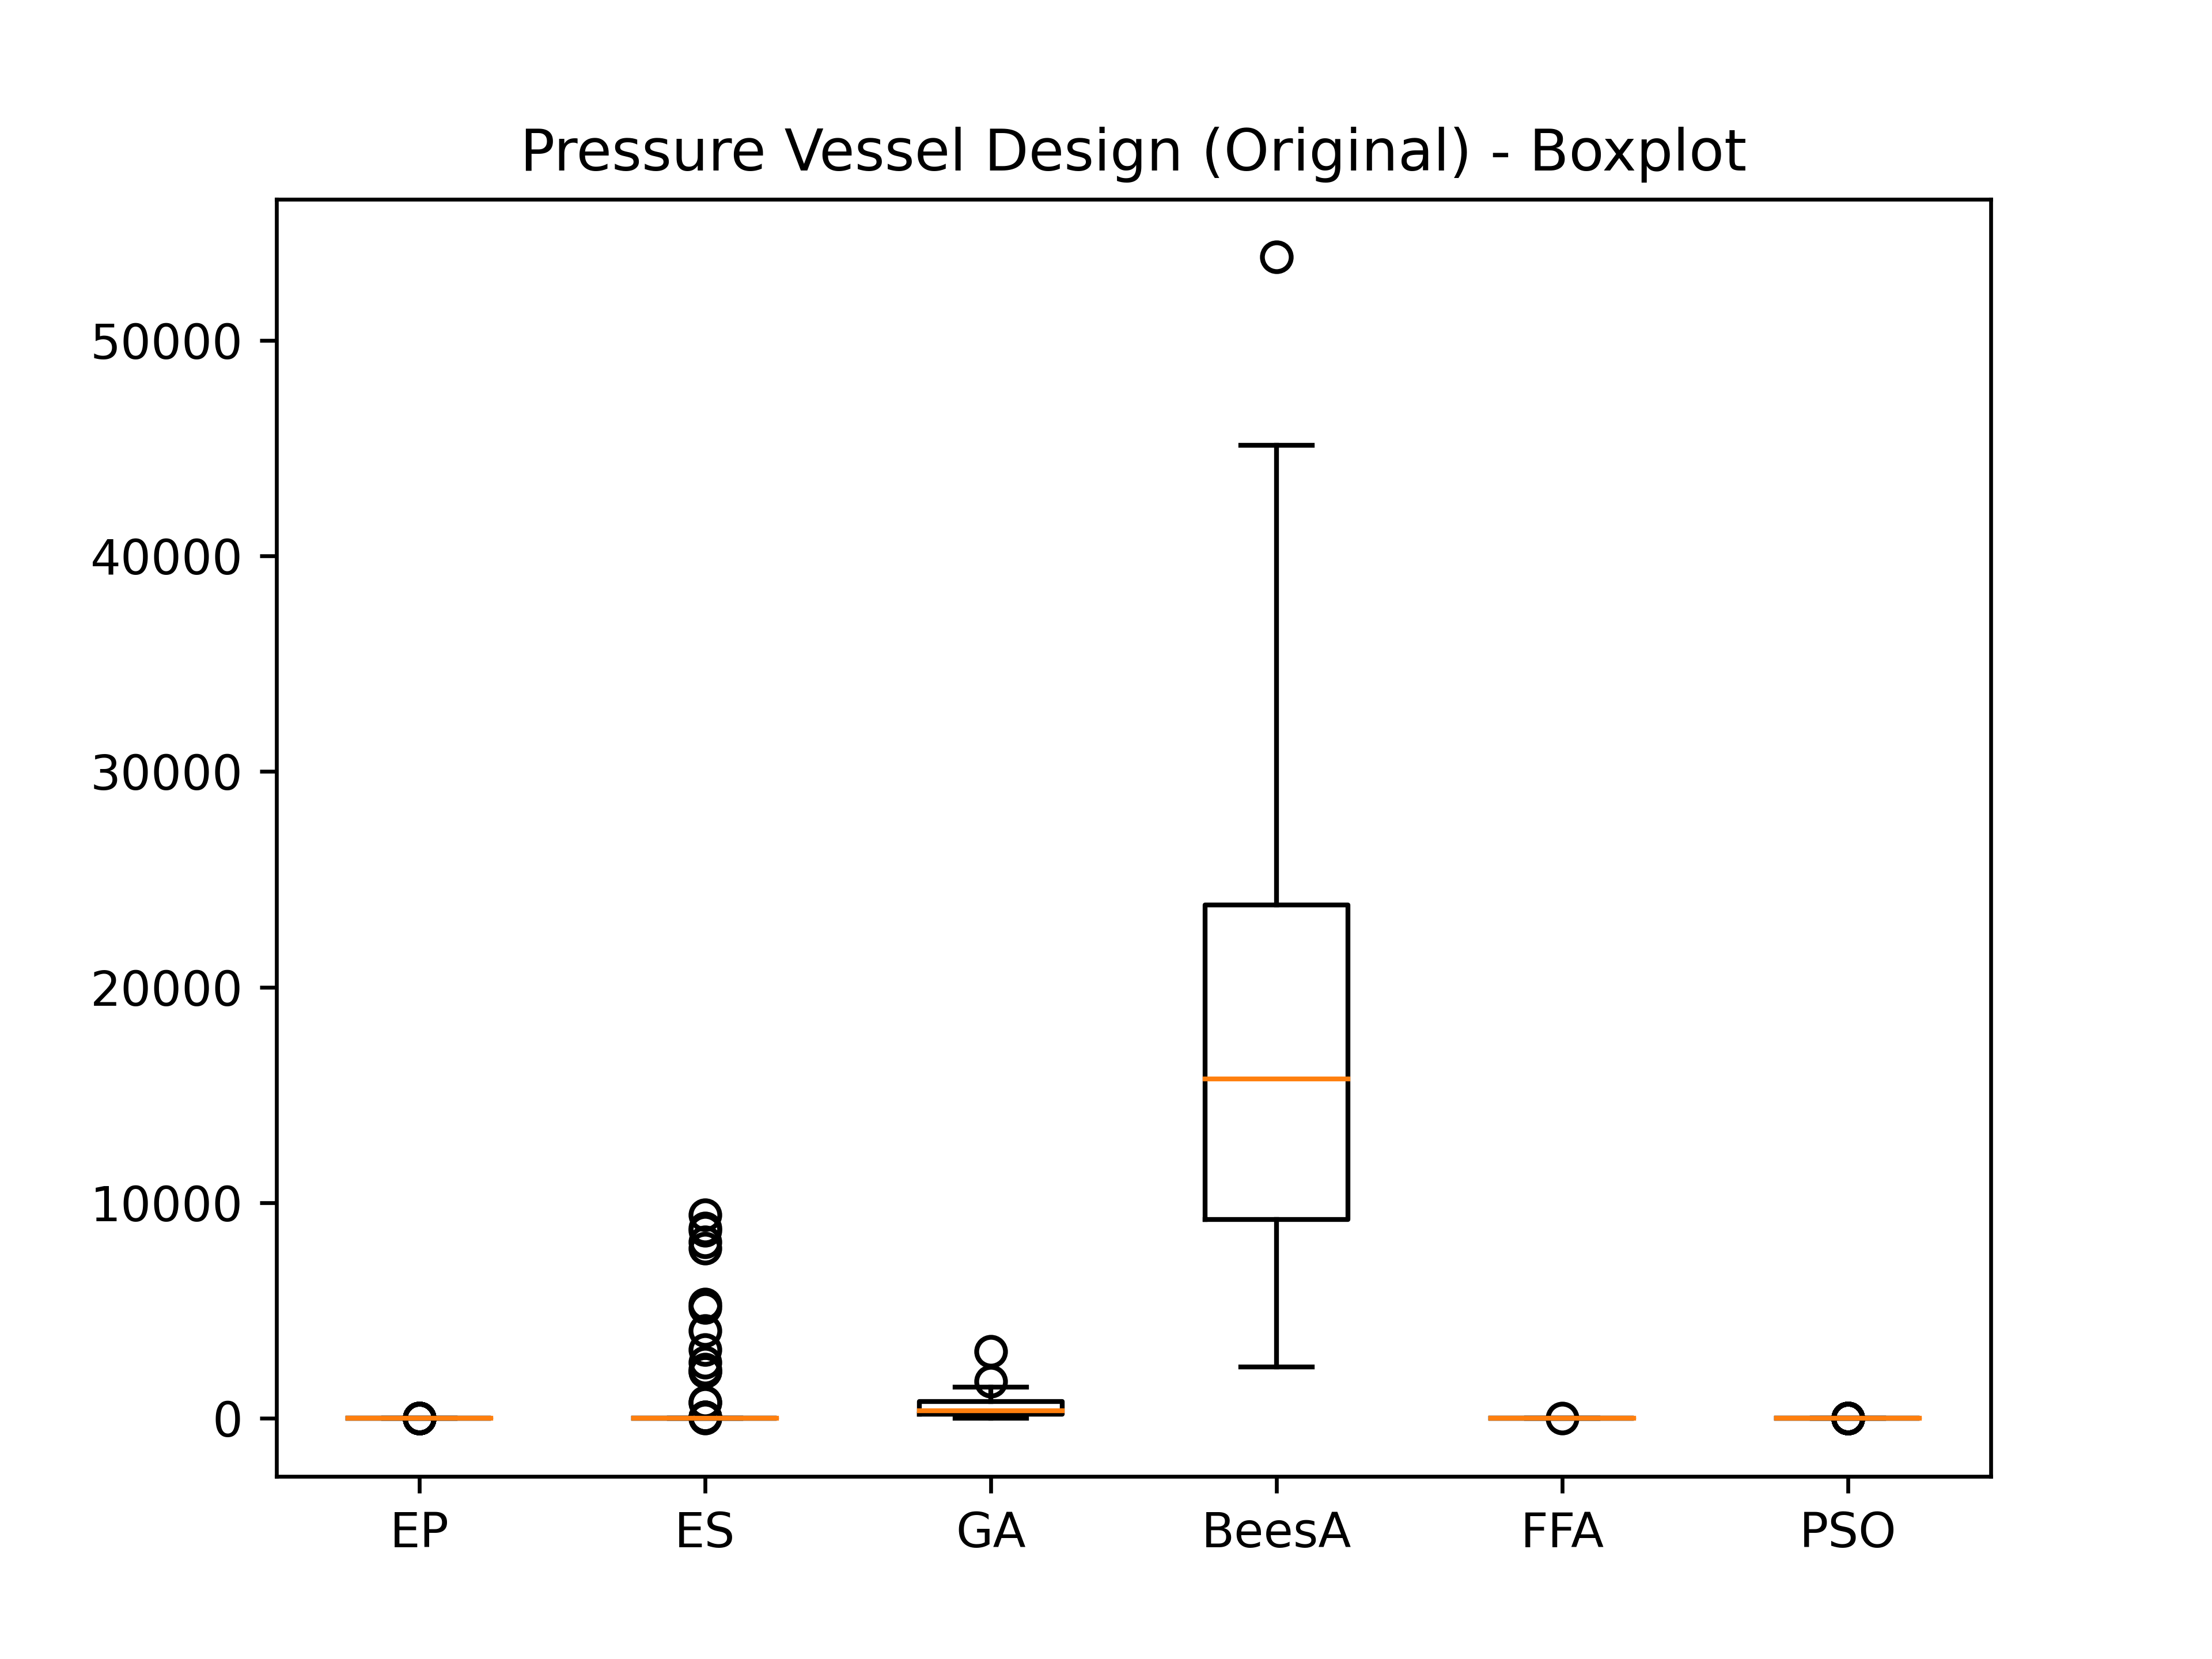
\includegraphics[scale=0.5]{images/pressure_vessel_problem_original_boxplot.png}
\end{figure}

Again, as it can be seen on the boxplot, there are no stability guaranteed for solution
in any algorithms.



Figure~\ref{fig:pressure_vessel_problem_original_convergence} shows the
function maximum, minimum and mean function of algorithm's evolution:

\begin{figure}[H]
\centering
\caption{Convergence lines for Pressure Vessel Design (Original)}
\label{fig:pressure_vessel_problem_original_convergence}
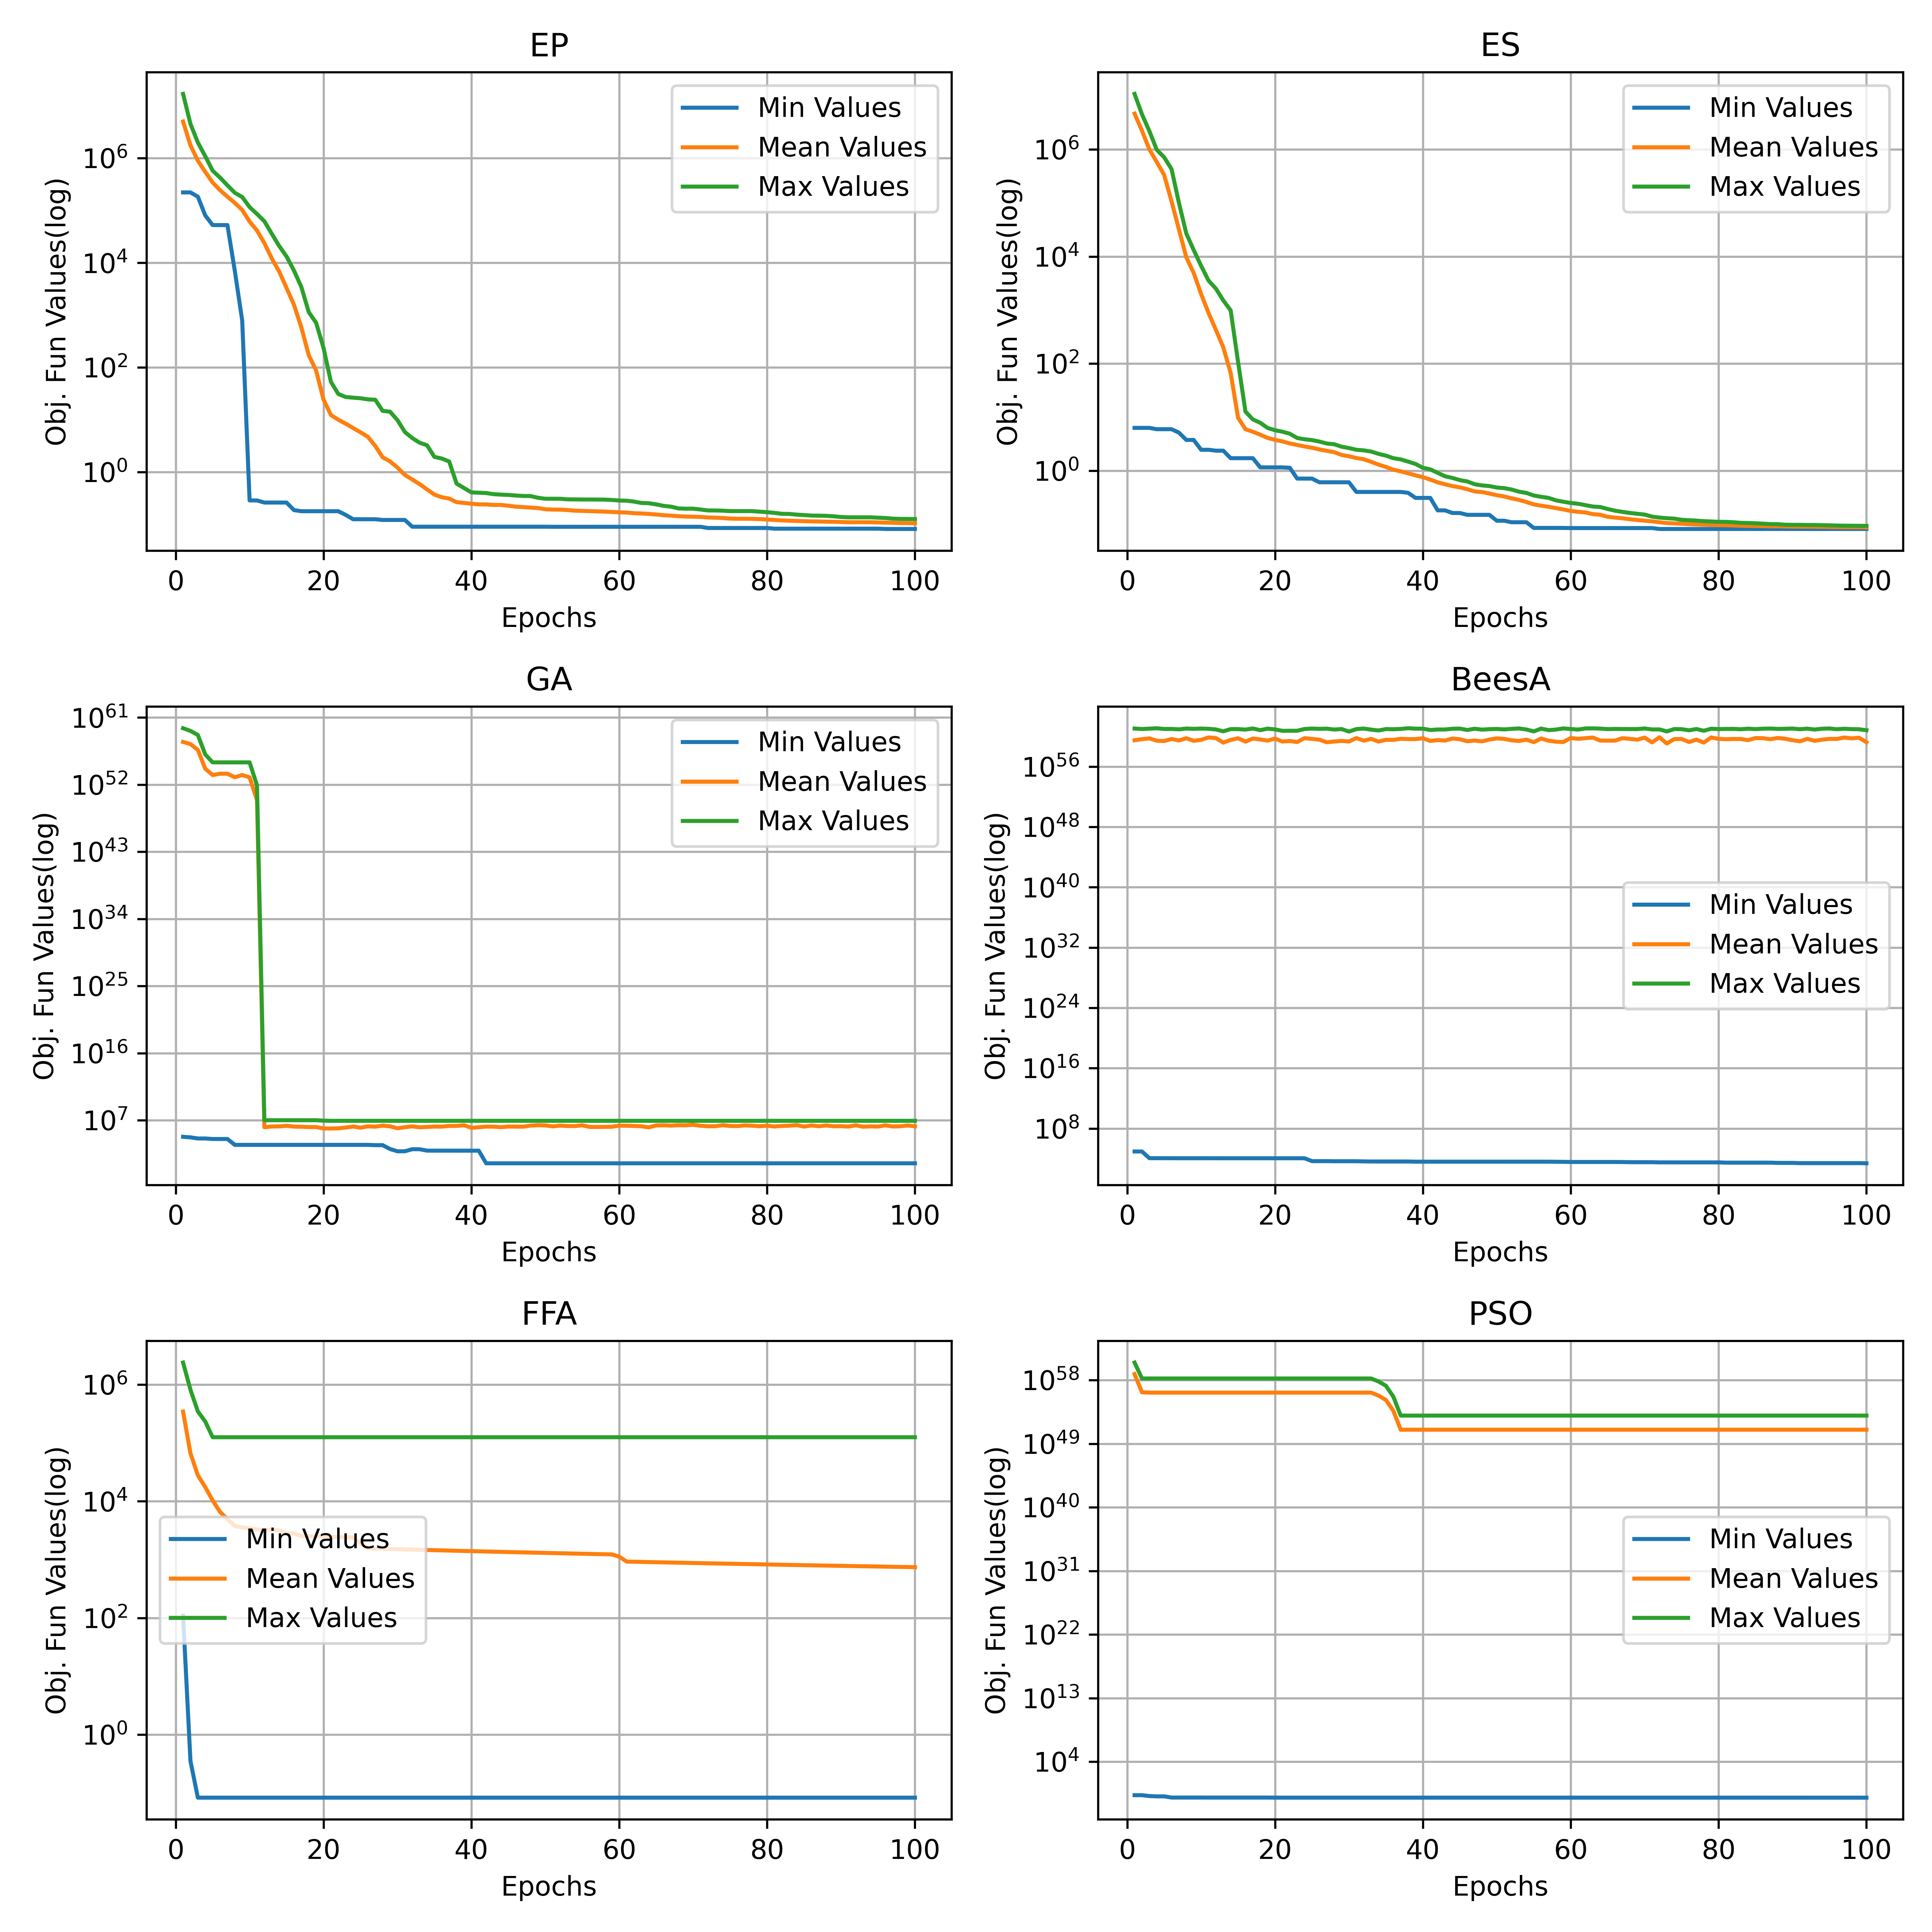
\includegraphics[width=0.4 \textwidth]{images/pressure_vessel_problem_original_convergence.png}
\end{figure}

All algorithms tested have slow evolution for the original variable boundings, as it is shown in the convergence evolution.



\subsection{Pressure Vessel Design}
\label{subsec:pressure_vessel_problem}

In this section are presented the results for a tweaked variable boundings of Pressure Vessel Design,
as exposed in Section~\ref{subsubsec:methodology-pressure-vessel-design}.

The best results for all algorithms are presented in Table~\ref{best_fits:pressure_vessel_problem}:

\begin{table}[H]
\centering
\caption{Best Fits for Pressure Vessel Design}
\label{best_fits:pressure_vessel_problem}
\resizebox{\columnwidth}{!}{%
\begin{tabular}{lrrrrr}
\toprule
Algorithm &      $x_1$ &      $x_2$ &       $x_3$ &        $x_4$ &         $f_x$ \\
\midrule
       EP & 0.75000000 & 0.35000000 & 40.68318345 & 195.00000000 & 5534.57345496 \\
       ES & 0.75000000 & 0.35000000 & 40.68322151 & 195.00000000 & 5534.57917966 \\
       GA & 0.75000816 & 0.35003661 & 40.68379662 & 195.00019653 & 5534.83662424 \\
    BeesA & 0.75000000 & 0.35000000 & 40.68319525 & 195.00000000 & 5534.57516657 \\
      FFA & 0.75000000 & 0.35000000 & 40.68318772 & 195.00000000 & 5534.57401617 \\
      PSO & 0.75000000 & 0.35000000 & 40.68318348 & 195.00000000 & 5534.57345480 \\
\bottomrule
\end{tabular}}
\end{table}

It is noticeable in this table that the best results and the best minimizers are quite the same,
so it cannot be said that all algorithms will solve the problem from this standpoint.




Another view of the solutions are presented in Table~\ref{function_values:pressure_vessel_problem}, where
are summarized the statistics of all 100 possible solutions for different starting points.

\begin{table}[H]
\centering
\caption{Statistical Information about function values for Pressure Vessel Design}
\resizebox{\columnwidth}{!}{%
\label{function_values:pressure_vessel_problem}
\begin{tabular}{lrrrrr}
\toprule
Algorithm &         Min F &        Mean F &      Median F &         Max F &   StdDev F \\
\midrule
       EP & 5534.57345496 & 5534.63426098 & 5534.61416291 & 5534.92993607 & 0.05804548 \\
       ES & 5534.57917966 & 5535.28165367 & 5535.06149254 & 5538.03003895 & 0.65098467 \\
       GA & 5534.83662424 & 5538.36788889 & 5536.92932748 & 5550.91639342 & 3.57079951 \\
    BeesA & 5534.57516657 & 5537.97495231 & 5537.04824684 & 5548.55587234 & 3.28239740 \\
      FFA & 5534.57401617 & 5534.58849395 & 5534.58435493 & 5534.63296149 & 0.01341777 \\
      PSO & 5534.57345480 & 5534.57381593 & 5534.57355270 & 5534.57625290 & 0.00053848 \\
\bottomrule
\end{tabular}}
\end{table}

It is hard to see any statistical  difference looking at any value in the table except standard deviation.
GA and BeesA seems to have the worst solutions, and EP, FFA and PSO seems to have a well defined behavior
since they have the lowest standard deviations, that is, all the solutions don't spread too much from each
other.


A quick way to access the Table~\ref{function_values:pressure_vessel_problem} is shown on Figure~\ref{fig:pressure_vessel_design_boxplot}.

\begin{figure}[H]
\centering
\caption{Boxplot for Pressure Vessel Design}
\label{fig:pressure_vessel_design_boxplot}
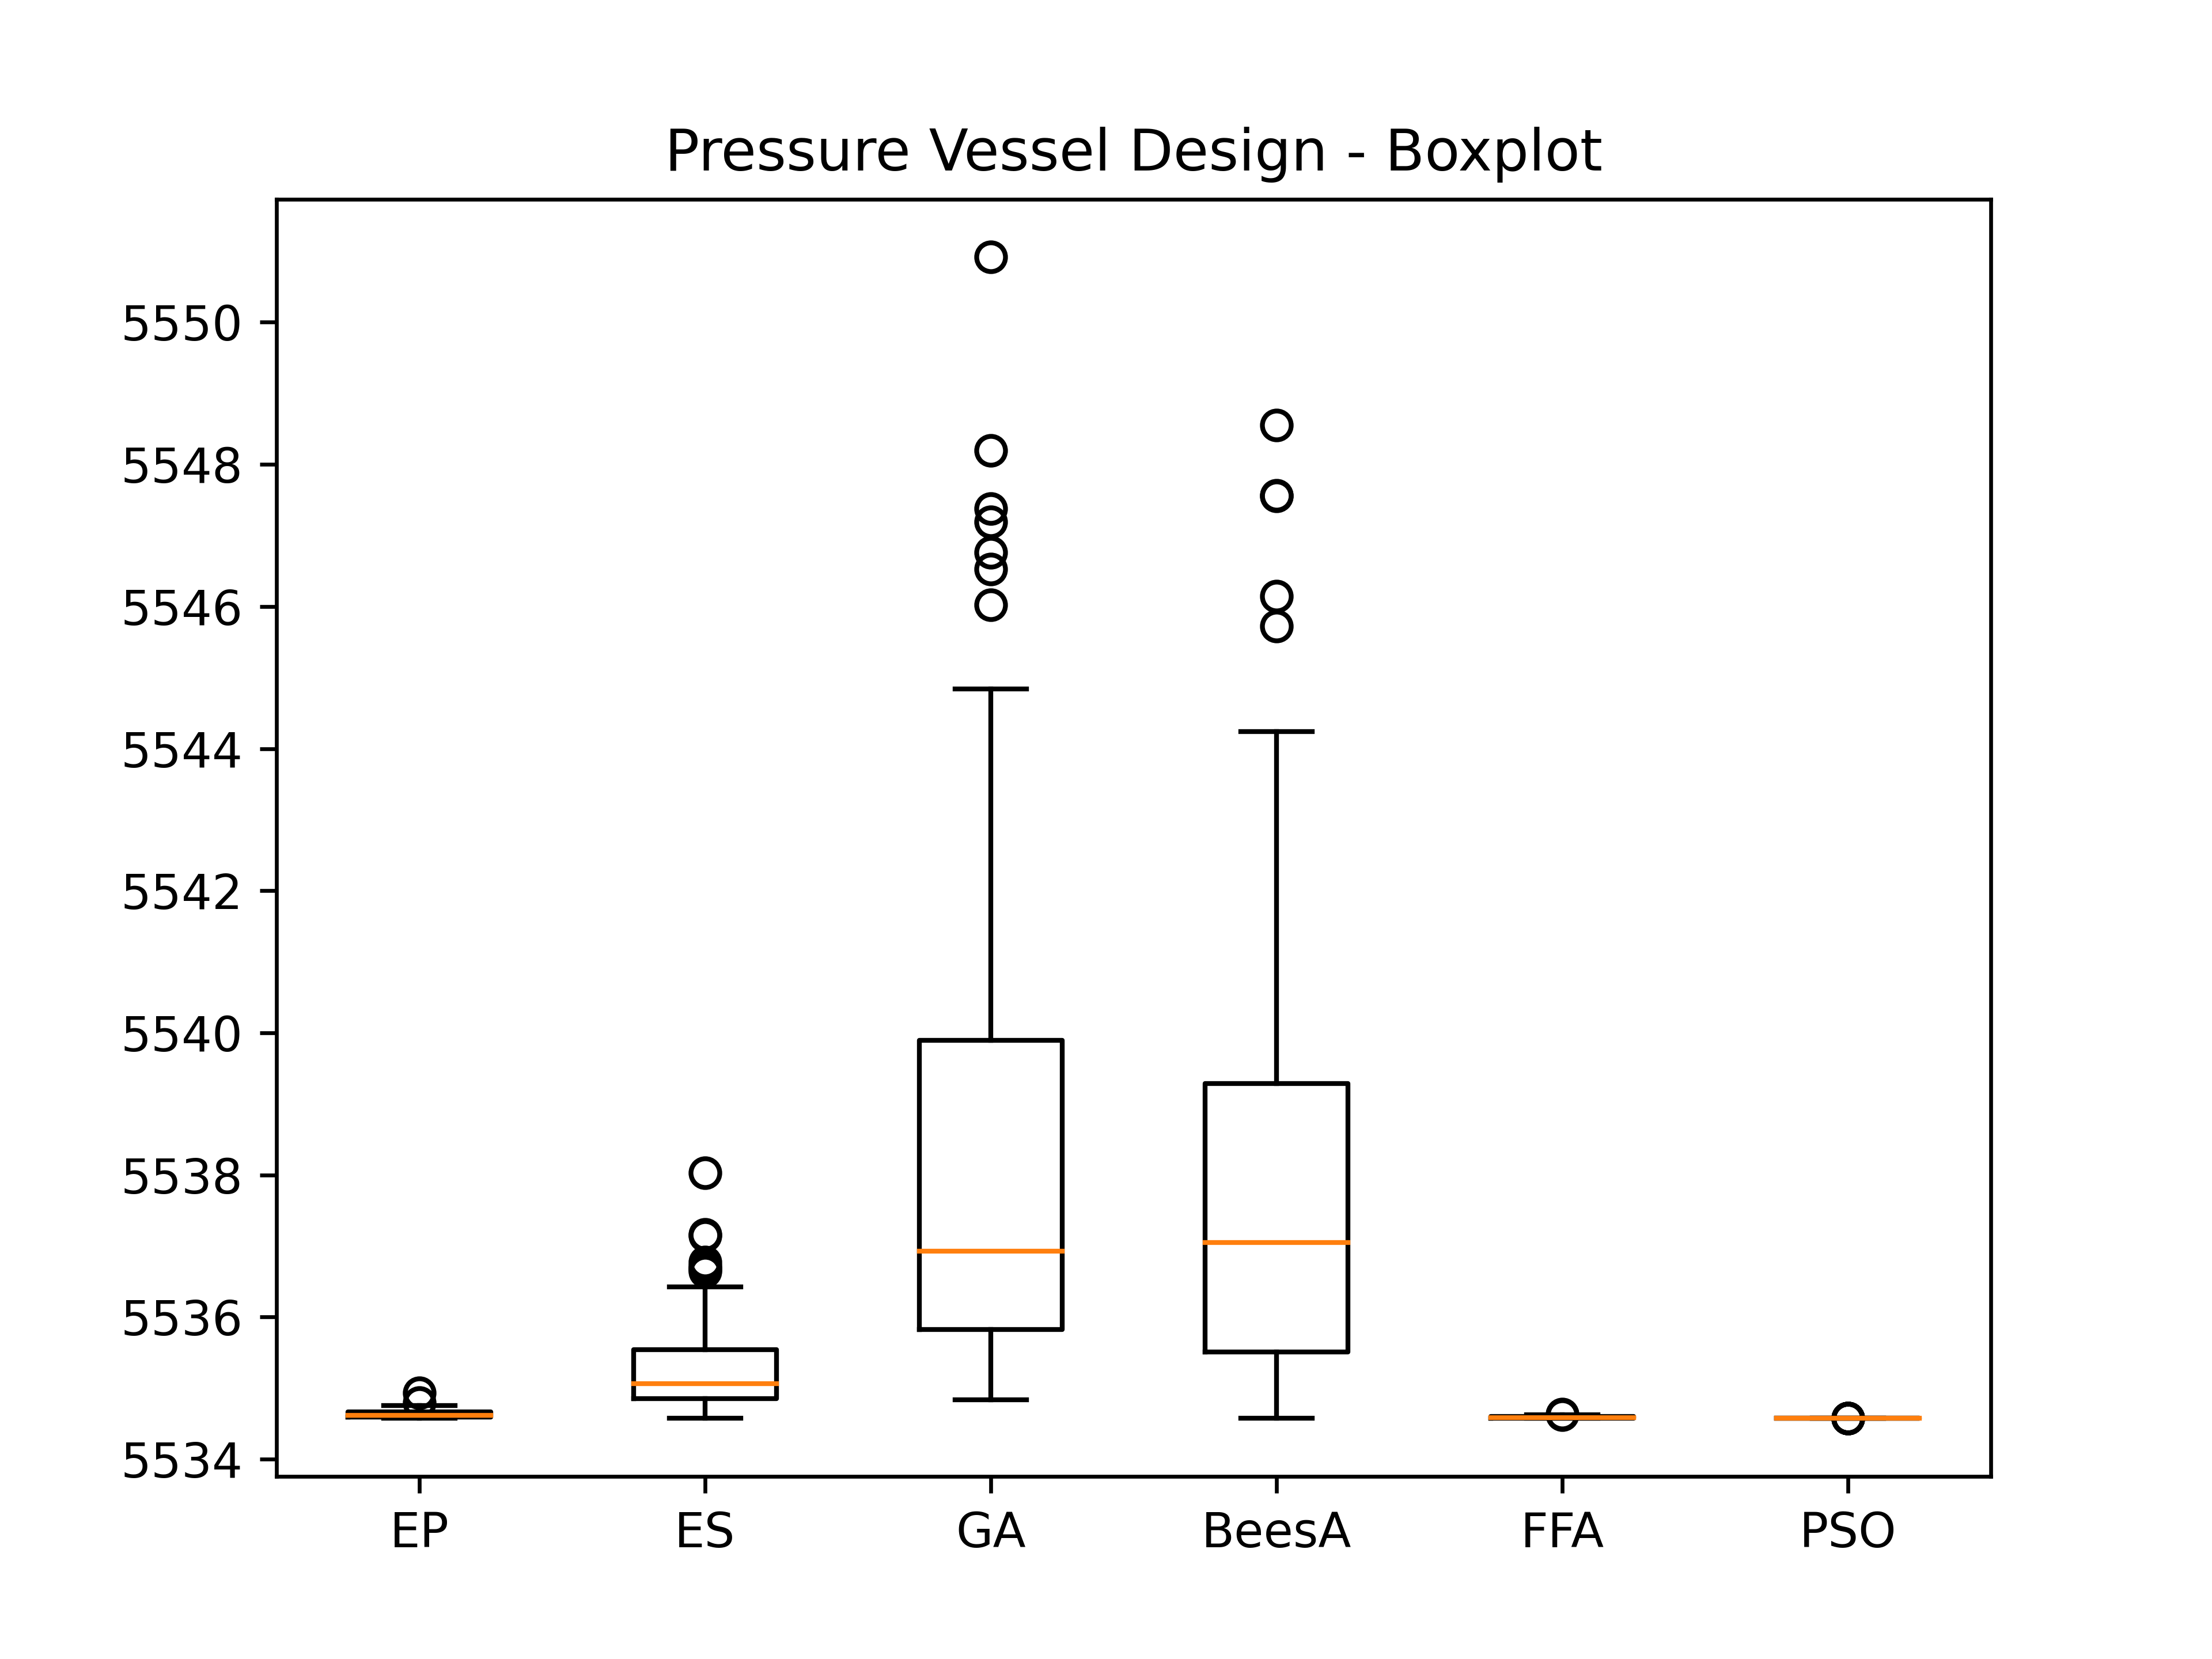
\includegraphics[scale=0.5]{images/pressure_vessel_problem_boxplot.png}
\end{figure}

It shows the same information as the Table~\ref{function_values:pressure_vessel_problem}
and it evidences that not all algorithms have the same mean, so it is a clear evidence
that not all algorithm give similar results from an arbitrary starting point (population).



Figure~\ref{fig:pressure_vessel_problem_convergence} shows the
function maximum, minimum and mean function of algorithm's evolution:

\begin{figure}[H]
\centering
\caption{Convergence lines for Pressure Vessel Design}
\label{fig:pressure_vessel_problem_convergence}
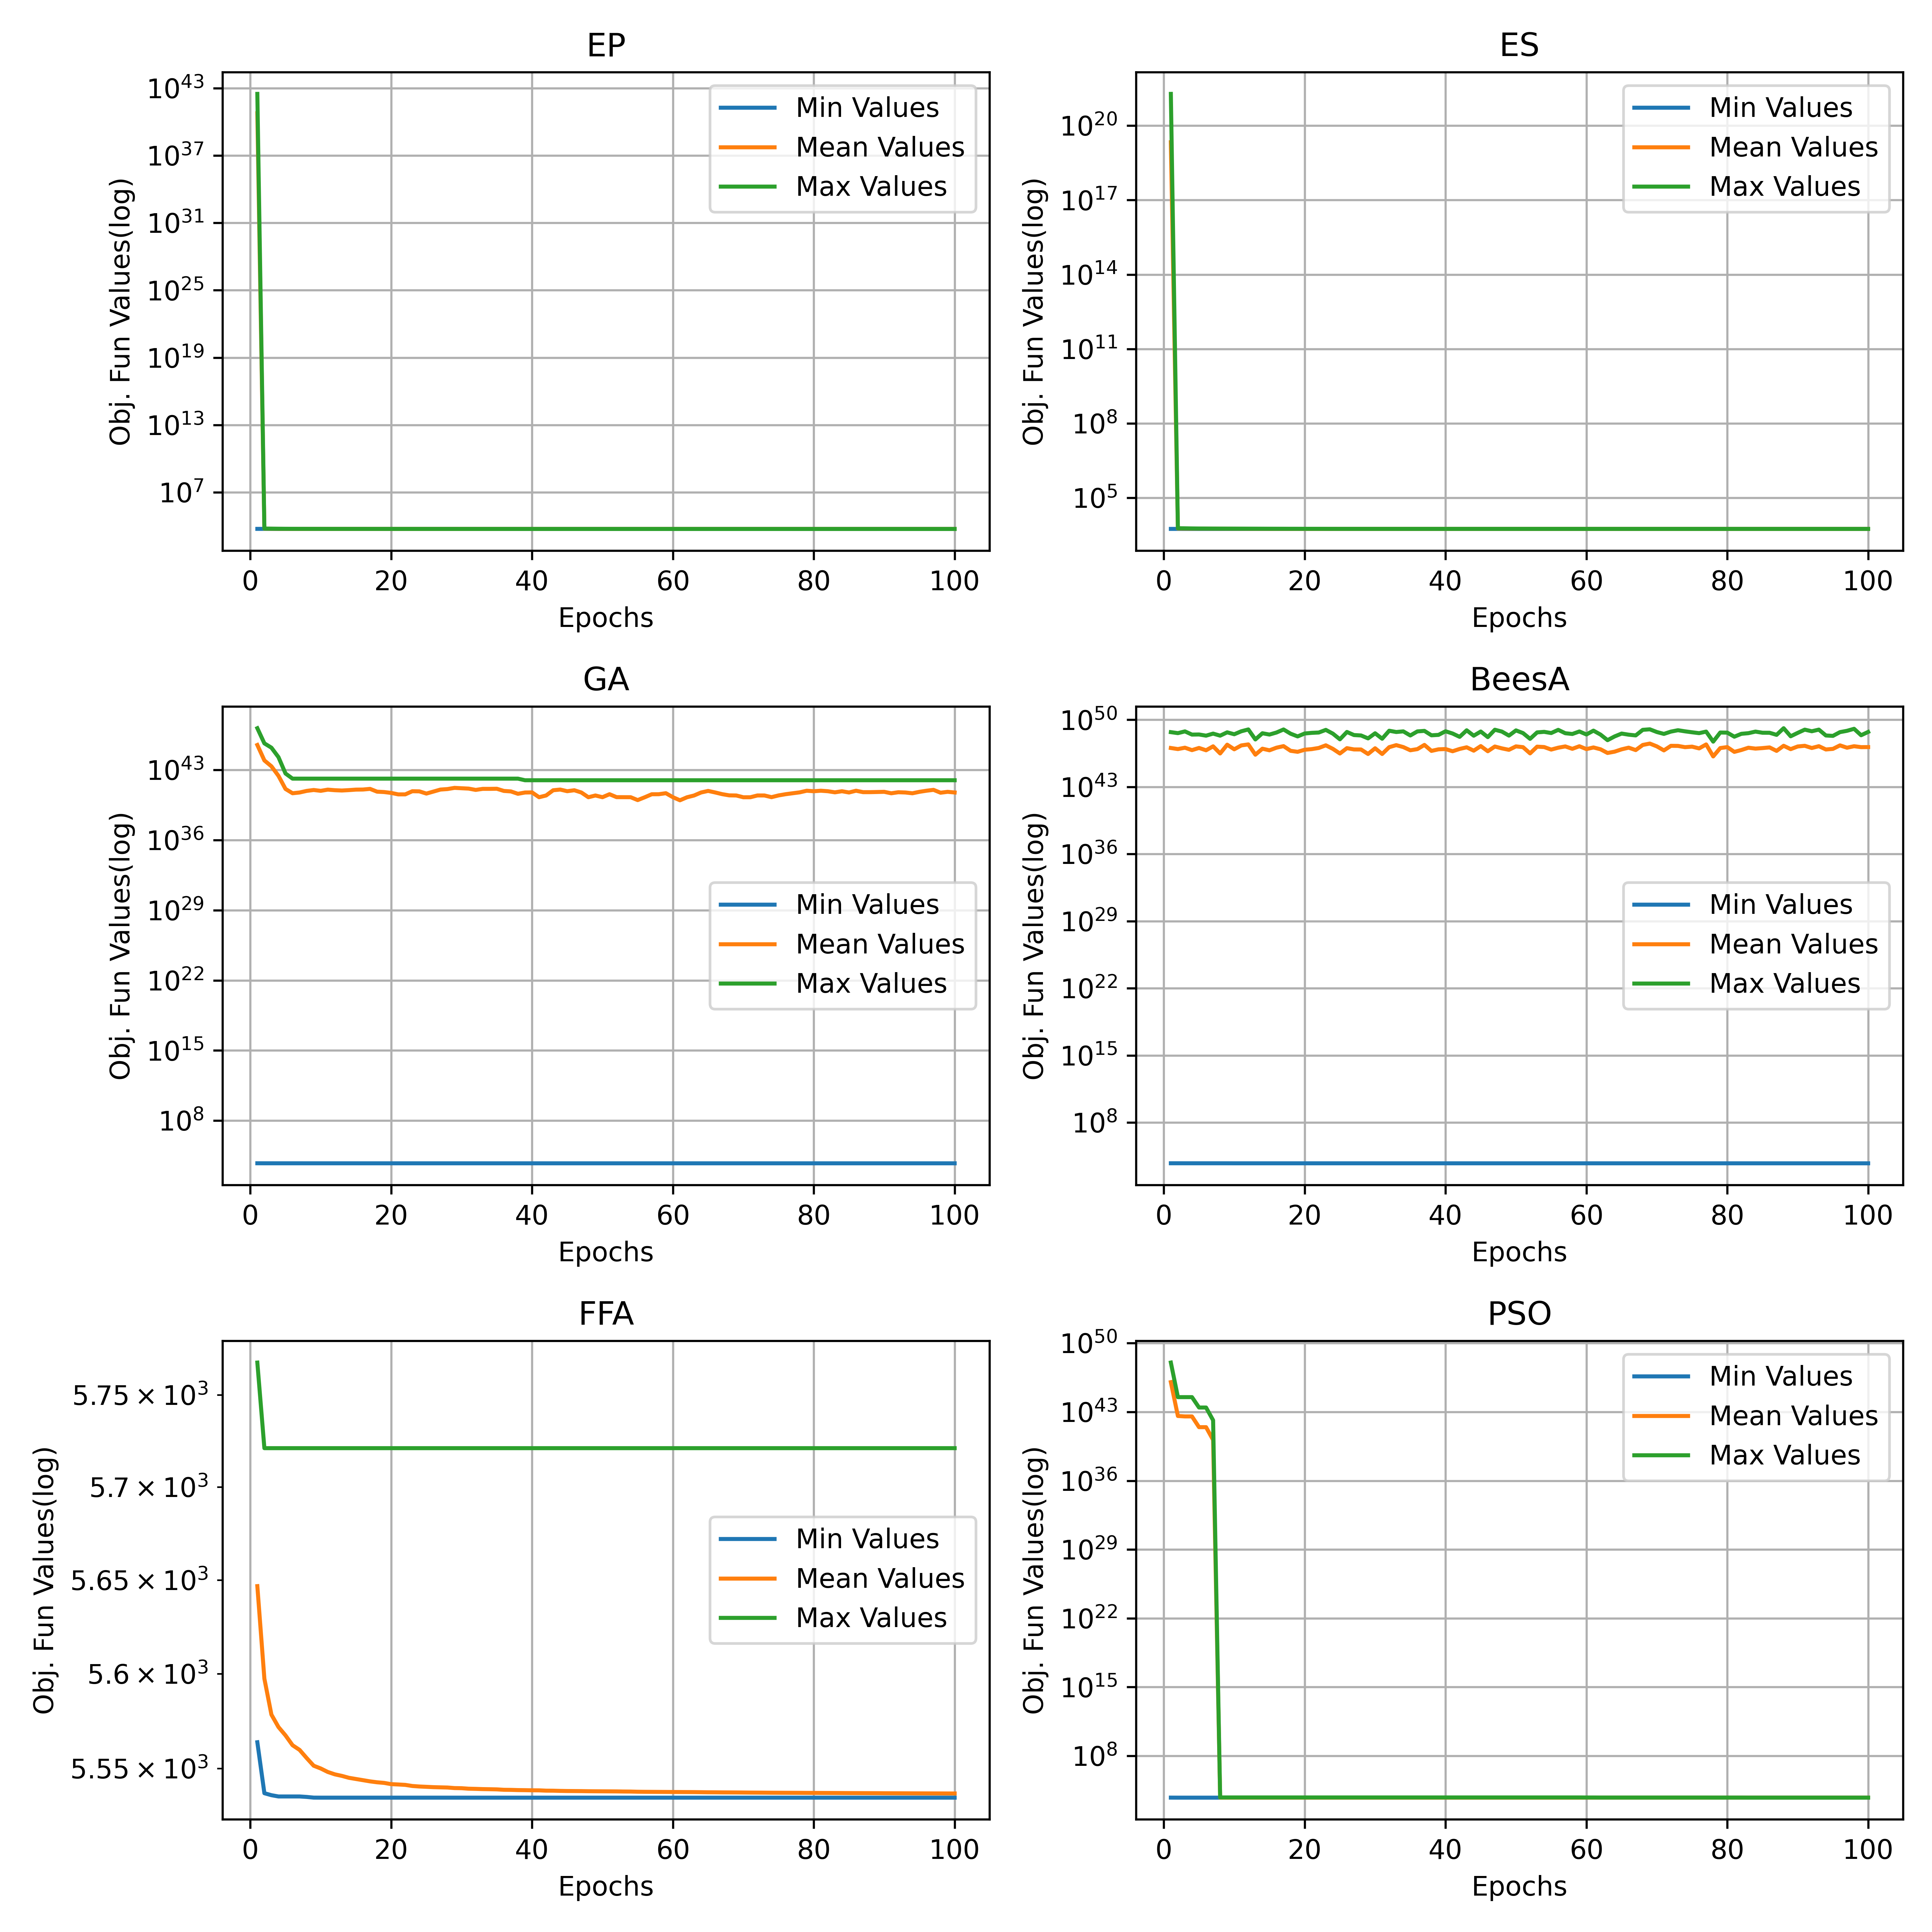
\includegraphics[width=0.4 \textwidth]{images/pressure_vessel_problem_convergence.png}
\end{figure}

EP, ES and PSO quickly converges all the solution once it find a viable minimum, whe GA, BeesA and FFA
maintain exploration and exploitation for all the epochs.
From Table~\ref{function_values:pressure_vessel_problem},
PSO has the best solution stability for the proud-and-lame-homemade custom bounding problem.


\subsection{Spring Tension Design}
\label{ssubec:spring_problem}

In this section are presented the results of Spring Tension Design optimization,
as exposed in Section~\ref{subsubsec:methodology-spring-tension-design}.

The best results for all algorithms are presented in Table~\ref{best_fits:spring_problem}:

\begin{table}[H]
\centering
\caption{Best Fits for Spring Tension Design}
\label{best_fits:spring_problem}
\resizebox{\columnwidth}{!}{%
\begin{tabular}{lrrrr}
\toprule
Algorithm &      $x_1$ &      $x_2$ &       $x_3$ &      $f_x$ \\
\midrule
       EP & 0.05078716 & 0.34120356 & 11.93931414 & 0.01250534 \\
       ES & 0.05000000 & 0.32292194 & 13.26929635 & 0.01252956 \\
       GA & 0.05260626 & 0.38419911 &  9.63922108 & 0.01252305 \\
    BeesA & 0.05141008 & 0.35564113 & 11.06109433 & 0.01250200 \\
      FFA & 0.05148403 & 0.35770175 & 10.95787946 & 0.01249803 \\
      PSO & 0.05000000 & 0.32241990 & 13.31368880 & 0.01252626 \\
\bottomrule
\end{tabular}}
\end{table}

Although the best fit points have noticeable differences, the cost function $f_x$ have similar results, that is, the
function $f_x$ seems to have weak minimal points.




Another view of the solutions are presented in Table~\ref{function_values:spring_problem}, where
are summarized the statistics of all 100 possible solutions for different starting points (populations).

\begin{table}[H]
\centering
\caption{Statistical Information about function values for Spring Tension Design}
\label{function_values:spring_problem}
\resizebox{\columnwidth}{!}{%
\begin{tabular}{lrrrrr}
\toprule
Algorithm &      Min F &     Mean F &   Median F &      Max F &   StdDev F \\
\midrule
       EP & 0.01250534 & 0.01255960 & 0.01253156 & 0.01453933 & 0.00020190 \\
       ES & 0.01252956 & 0.01281857 & 0.01274283 & 0.01346214 & 0.00024181 \\
       GA & 0.01252305 & 0.01628575 & 0.01616768 & 0.02561808 & 0.00273276 \\
    BeesA & 0.01250200 & 0.01268010 & 0.01261691 & 0.01406679 & 0.00021629 \\
      FFA & 0.01249803 & 0.01254780 & 0.01253499 & 0.01268116 & 0.00003152 \\
      PSO & 0.01252626 & 0.01390866 & 0.01318774 & 0.03036537 & 0.00342240 \\
\bottomrule
\end{tabular}}
\end{table}

Looking at standard deviation, EP, ES and BeesA appear to have the same distribution;
FFA has the lowest function value spread around the mean; GA and PSO have the largest
function values spread around the mean and particularly GA tend to give discrepant results
that the rest.


A quick way to access the Table~\ref{function_values:spring_problem} is
shown on Figure~\ref{fig:spring_tension_design_boxplot}.

\begin{figure}[H]
\centering
\caption{Boxplot for Spring Tension Design}
\label{fig:spring_tension_design_boxplot}
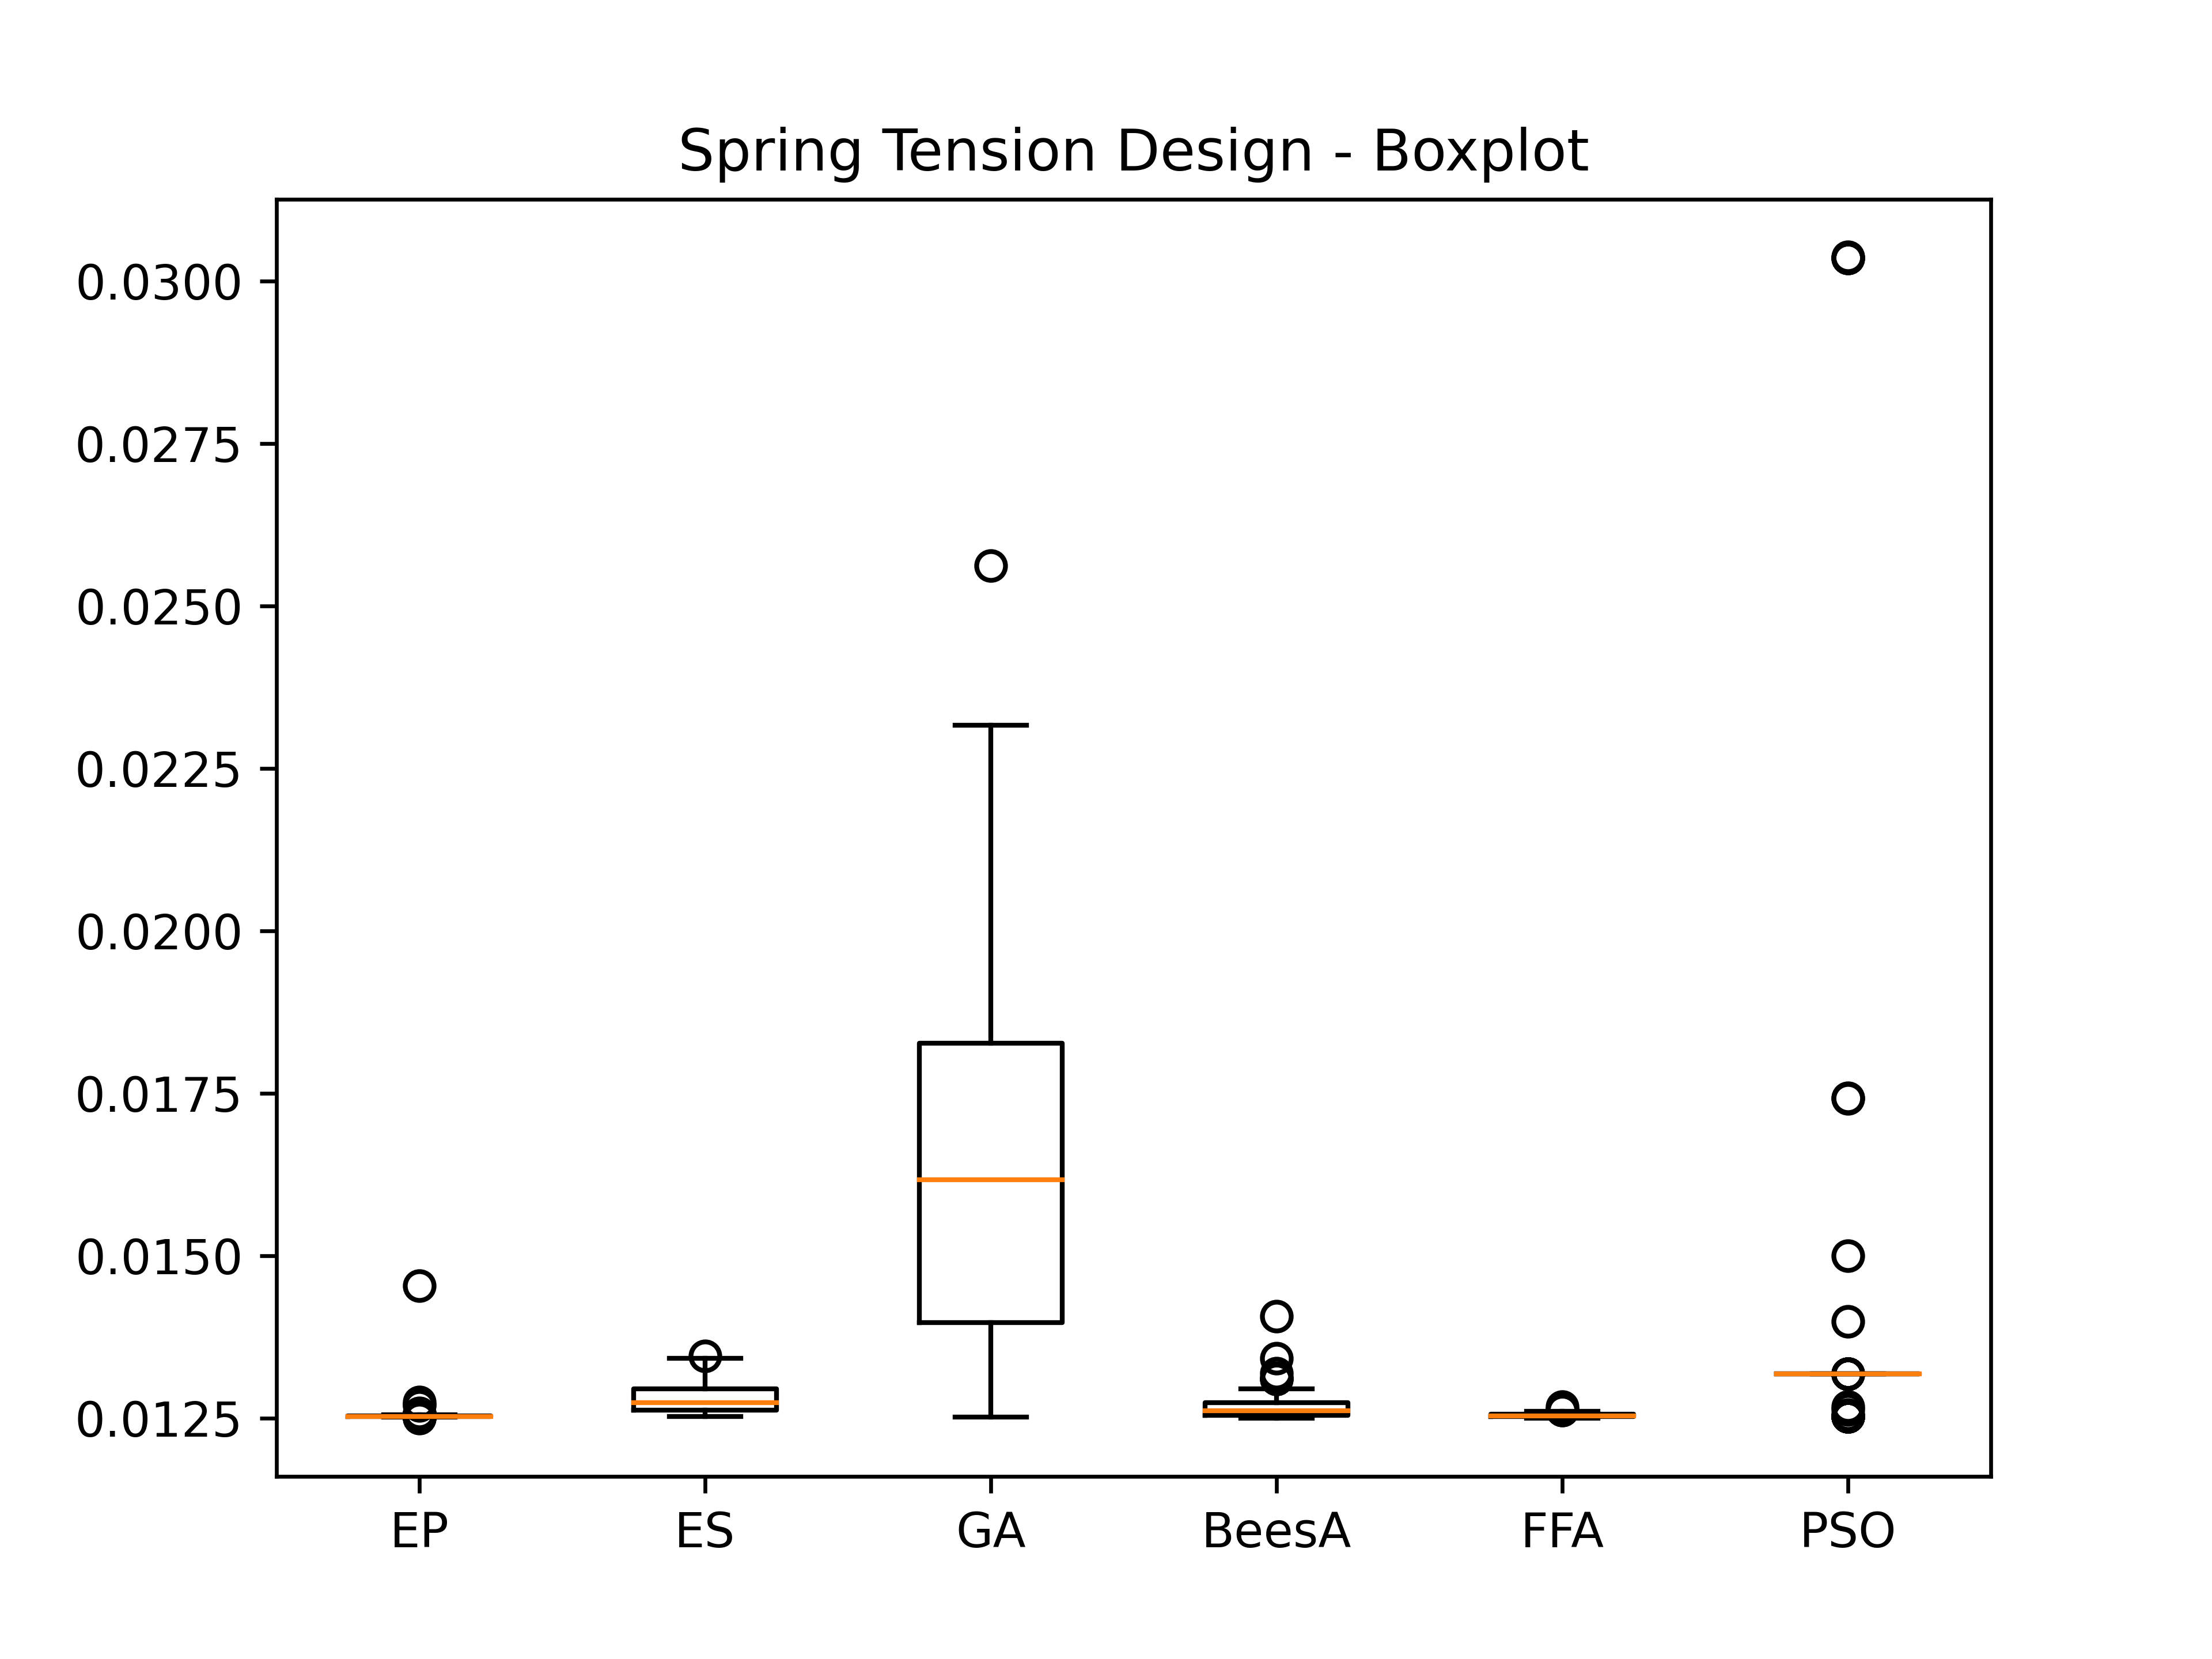
\includegraphics[scale=0.5]{images/spring_problem_boxplot.png}
\end{figure}

It shows the same information as the Table~\ref{function_values:spring_problem}
and it evidences that not all algorithms have the same mean, so it is a clear evidence
that not all algorithm give similar results from an arbitrary starting point (population).

Figure~\ref{fig:spring_problem_convergence} shows the
function maximum, minimum and mean function of algorithm's evolution:

\begin{figure}[H]
\centering
\caption{Convergence lines for Spring Tension Design}
\label{fig:spring_problem_convergence}
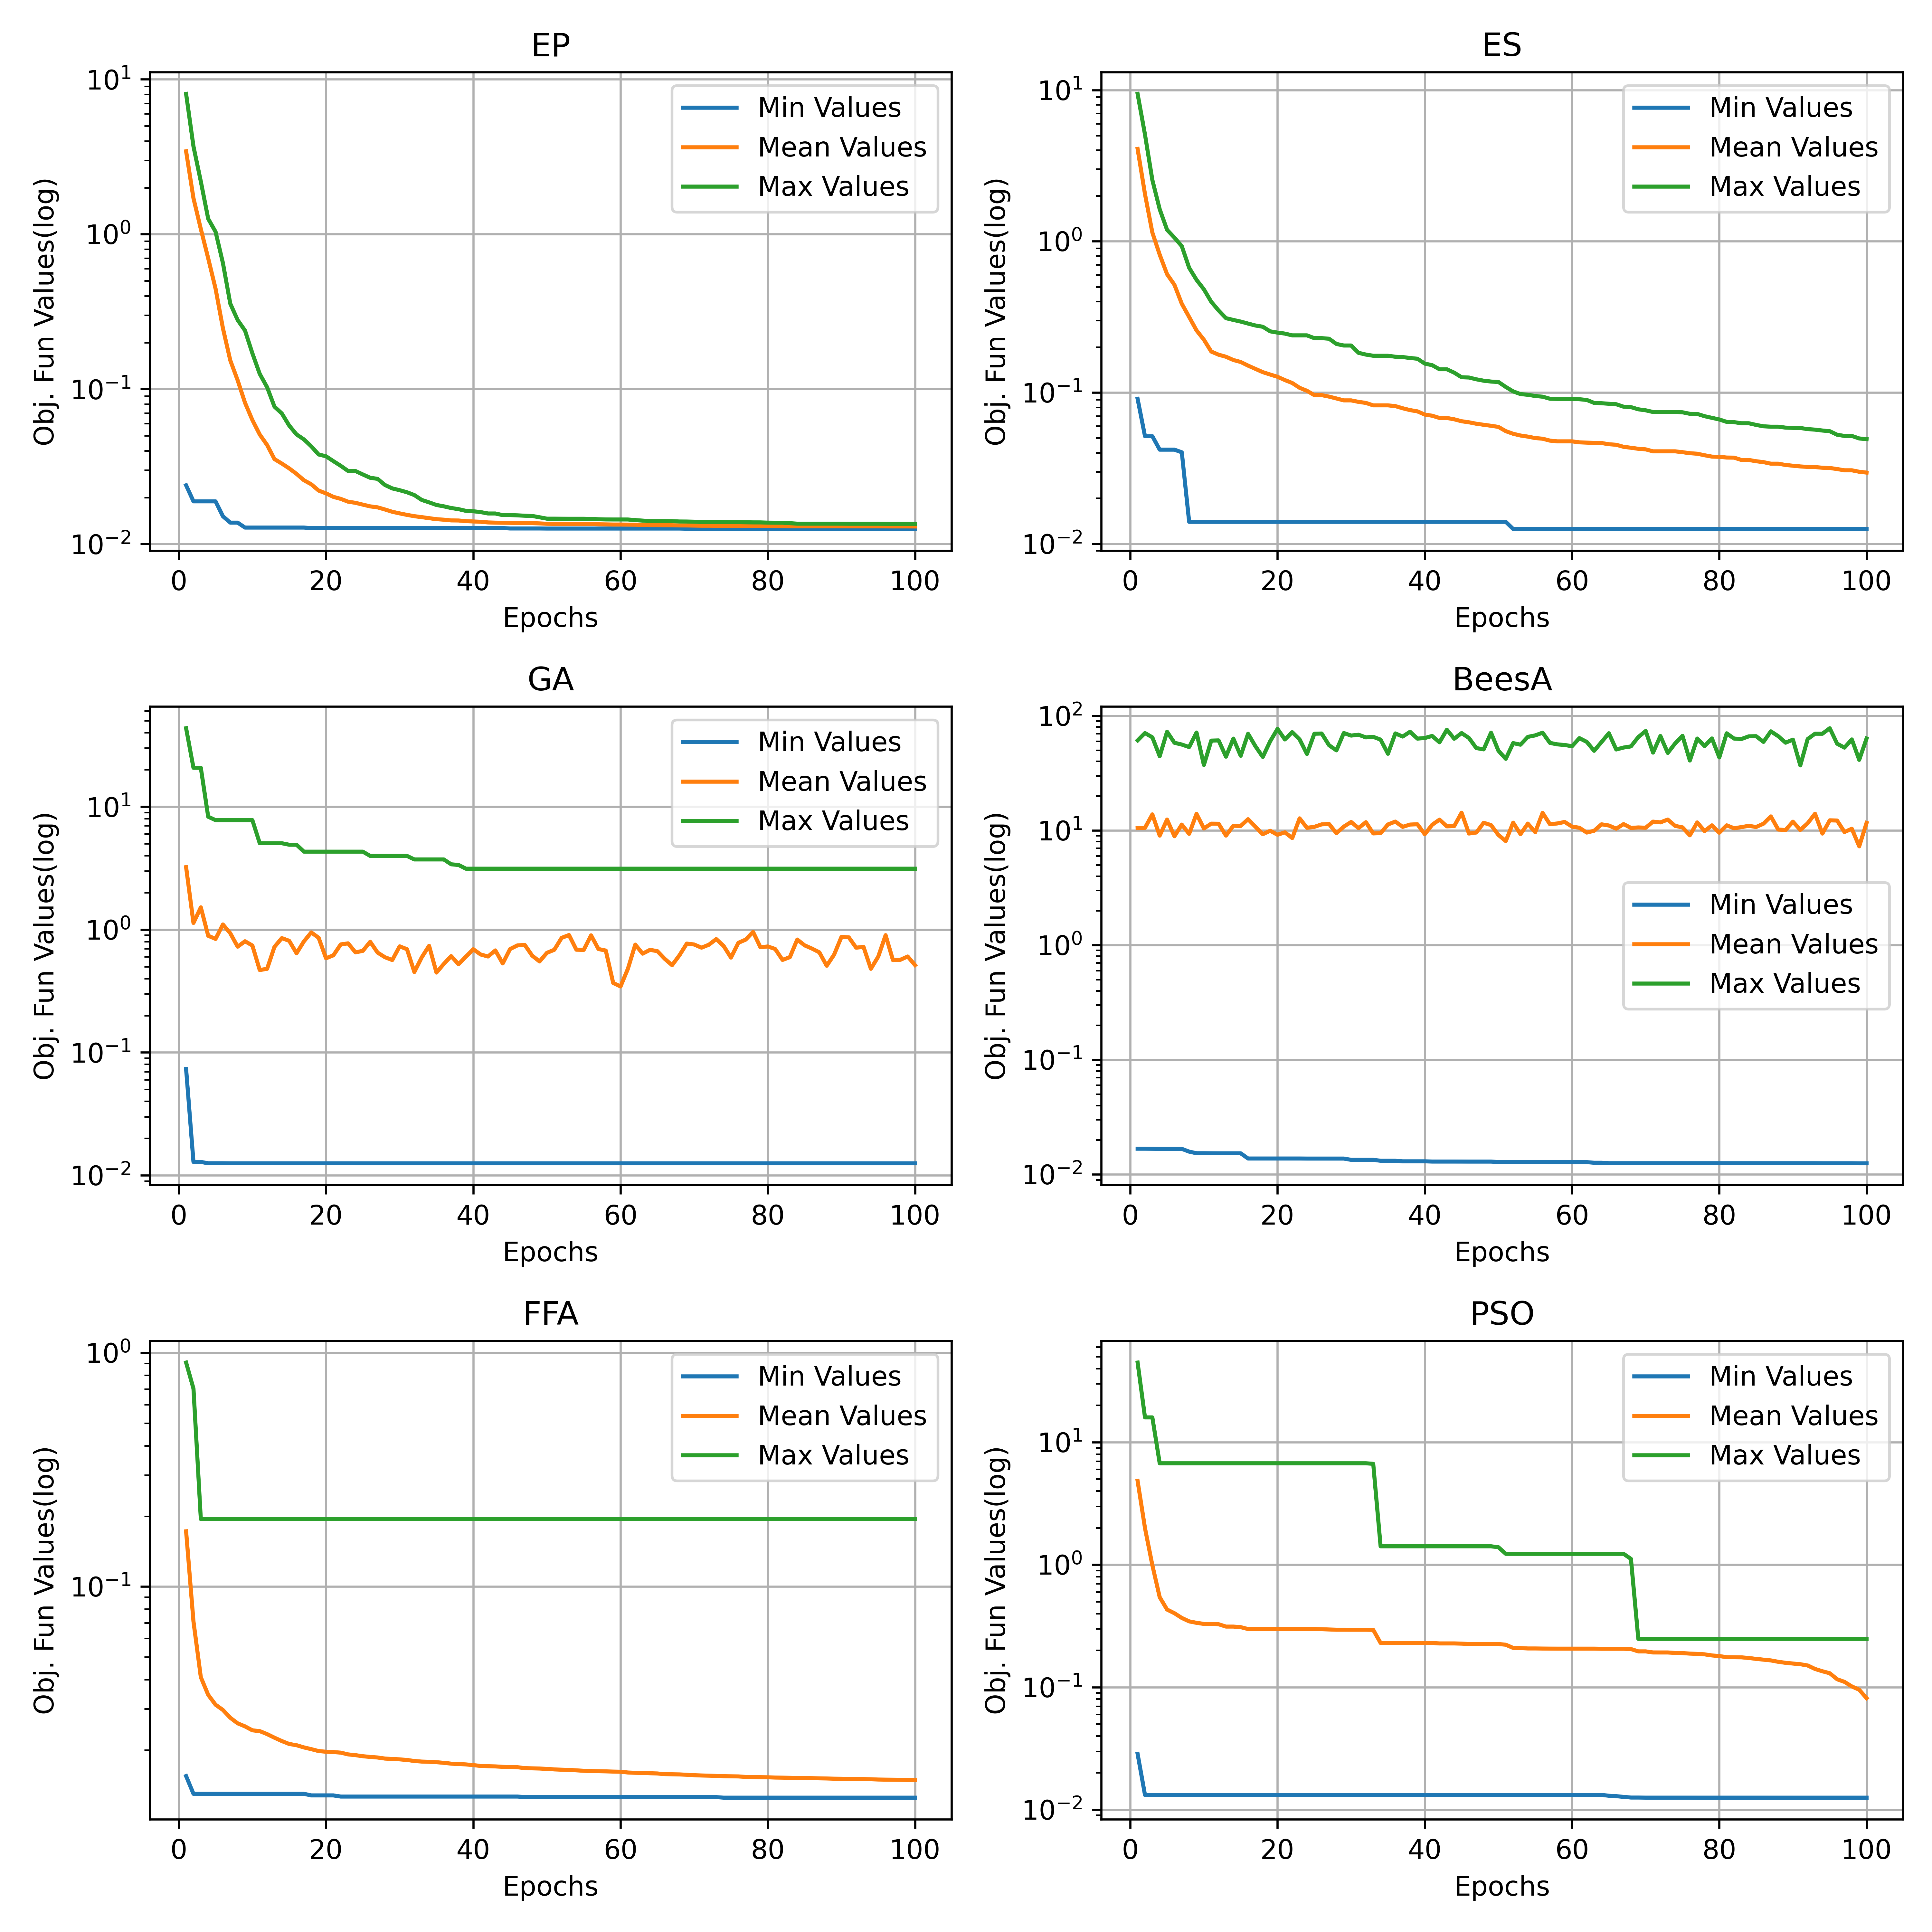
\includegraphics[width=0.4 \textwidth]{images/spring_problem_convergence.png}
\end{figure}

EP, ES and FFA have the best fitness.
All algorithms seems to converge the minimum line very quickly when
the algorithm find a minimal point.
Apart from EP and ES, the algorithms seems to maintain exploration and exploitation
until the time runs out.


\subsection{Significance Test}
\label{subsec:pressure_vessel_problem_significance_test}

The Friedman test is the non-parametric test used to compare related sample data, that is,
when the same individual is evaluated more than once.
The Friedman test does not use the data numbers directly, but the ranks occupied by
them after the sorting done for each group separately. After sorting, the hypothesis
of equality of the sum of the ranks of each group is tested.

Interpretation is as follows:
\begin{itemize}
    \item Assume two hypothesis about the data:
        \subitem $H_0$: The mean for each population is equal.
        \subitem $H_1$: At least one population mean is different from the rest.
    \item Given p-value, decide:
        \subitem p-value $\geq 0.05$: Reject $H_1$ with $95\%$ of confidence and accept null hypothesis;
        \subitem Accept $H_1$ otherwise.
\end{itemize}

The Table~\ref{friedman_test} resumes the Friedman's Chi-Squared Test made using
the 6 samples took by the algorithm's best results fore each run:

\begin{table}[H]
\centering
\caption{Significance Test Using Friedman Chi-Squared Test}
\label{friedman_test}
\resizebox{\columnwidth}{!}{%
\begin{tabular}{lrr}
\toprule
                          Problem &   Rank &    p-value \\
\midrule
Pressure Vessel Design (Original) & 425.07428571 & 0.00000000 \\
           Pressure Vessel Design & 436.16000000 & 0.00000000 \\
            Spring Tension Design & 339.05714286 & 0.00000000 \\
\bottomrule
\end{tabular}}
\end{table}

Using the interpretation rules, since the p-value is less than $0.05$, the null hypotesis $H_0$
is rejected and each problem have at least one population with different mean from the rest.
Thus, not all algorithms gives the same result for the same problem.


Developed by F. Wilcoxon in 1945, the paired Wilcoxon test is based on the ranks
of intrapair differences. This non-parametric test, used to compare related samples,
is an alternative to the Student t-test when samples do not follow a normal distribution.
Therefore, the Wilcoxon test is used to test whether sample medians are equal in cases
where the assumption of normality is not satisfied or when it is not possible to check
this assumption.

Interpretation is as follows:
\begin{itemize}
    \item Assume two hypothesis about the data:
        \subitem $H_0$: the distributions of both samples are equal;
        \subitem $H_1$: the distributions of both samples are not equal.
    \item Given p-value, decide:
        \subitem p-value $\leq 0.05$: Reject $H_1$ with $95\%$ of confidence and accept null hypothesis;
        \subitem Accept $H_1$ otherwise.
\end{itemize}

The Table~\ref{wilcoxon_test:pressure_vessel_problem_original} gives the Wilcoxon test results
for \textit{Pressure Vessel Design} using the original variables bounding as exposed in Section~\ref{subsubsec:methodology-pressure-vessel-design}.

\begin{table}[H]
\centering
\caption{Significance Test Using Wilcoxon Test for Pressure Vessel Design (Original)}
\label{wilcoxon_test:pressure_vessel_problem_original}
\resizebox{\columnwidth}{!}{%
\begin{tabular}{lllllll}
\toprule
  --- & EP & ES & GA & BeesA & FFA & PSO \\
\midrule
   EP & 0.0 & 1.20e-16 & 3.90e-18 & 3.90e-18 & 0.07 & 2.02e-4 \\
   ES & 1.20e-16 & 0.0 & 6.56-06 & 4.96e-18 & 5.49e-14 & 1.41e-17 \\
   GA & 3.90e-18 & 6.56e-06 & 0.0 & 3.90e-18 & 3.90e-18 & 3.90e-18 \\
BeesA & 3.90e-18 & 4.96e-18 & 3.90e-18 & 0.0 & 3.90e-18 & 3.90e-18 \\
  FFA & 0.07 & 5.49e-14 & 3.90e-18 & 3.90e-18 & 0.0 &  5.34e-05 \\
  PSO & 2.02e-4 & 1.41e-17 & 3.90e-18 &  3.90e-18 & 5.34e-05 & 0.0 \\
\bottomrule
\end{tabular}}
\end{table}

It is easy to notice that, from Wilcoxon test, FAA and EP have different distributions.
$H_1$ is only accepted in case of FFA and EP: they distributions seems to be not equal.

The Table~\ref{wilcoxon_test:pressure_vessel_problem} gives the Wilcoxon test results
for \textit{Pressure Vessel Design} using the proud-and-lame-homemade variables bounding
as exposed in Section~\ref{subsubsec:methodology-pressure-vessel-design}.


\begin{table}[H]
\centering
\caption{Significance Test Using Wilcoxon Test for Pressure Vessel Design}
\label{wilcoxon_test:pressure_vessel_problem}
\resizebox{\columnwidth}{!}{%
\begin{tabular}{lllllll}
\toprule
  --- & EP & ES & GA & BeesA & FFA & PSO \\
\midrule
   EP & 0.0 & 9.04e-18 & 3.90e-18 & 6.12e-18 & 8.79e-12 & 4.40e-18 \\
   ES & 9.04e-18 & 0.0 & 1.71e-14 & 1.64e-13 & 4.81e-18 & 3.90e-18 \\
   GA & 3.90e-18 & 1.71e-14 & 0.0 & 0.38 & 3.90e-18 & 3.90e-18 \\
BeesA & 6.12e-18 & 1.64e-13 & 0.38 & 0.0 & 4.30e-18 & 3.90e-18 \\
  FFA & 8.79e-12 & 4.81e-18 & 3.90e-18 & 4.30e-18 & 0.0 & 4.02e-18 \\
  PSO & 4.40e-18 & 3.90e-18 & 3.90e-18 & 3.90e-18 & 4.02e-18 & 0.0 \\
\bottomrule
\end{tabular}}
\end{table}

EP, ES, FAA and PSO appears to have the same distributions.
However, BeesA and GA appears to have different distributions.
This fact confirms the results found in Table~\ref{function_values:pressure_vessel_problem}.



The Table~\ref{wilcoxon_test:spring_problem} gives the Wilcoxon test results
for \textit{Spring Tension Design} as exposed in Section~\ref{subsubsec:methodology-spring-tension-design}.


\begin{table}[H]
\centering
\caption{Significance Test Using Wilcoxon Test for Spring Tension Design}
\label{wilcoxon_test:spring_problem}
\resizebox{\columnwidth}{!}{%
\begin{tabular}{lllllll}
\toprule
  --- & EP & ES & GA & BeesA & FFA & PSO \\
\midrule
   EP & 0.0 & 1.47e-16 & 4.01e-18 & 4.37e-12 & 0.01 & 2.33e-16 \\
   ES & 1.47e-16 & 0.0 &  1.90e-17 & 2.12e-06 & 3.24e-17 & 7.98e-12 \\
   GA & 4.01e-18 &  1.90e-17 & 0.0 & 8.02e-18 & 4.27e-18 & 1.29e-11 \\
BeesA & 4.36e-12 & 2.12e-06 & 8.02e-18 & 0.0 & 3.01e-11 & 6.82e-15 \\
  FFA & 0.01 & 3.23e-17 & 4.27e-18 & 3.01e-11 & 0.0 & 9.32e-18 \\
  PSO & 2.33e-16 & 7.98e-12 & 1.29e-11 & 6.82e-15 & 9.32e-18 & 0.0 \\
\bottomrule
\end{tabular}}
\end{table}

From Wilcoxon Test, the are no difference between all algorithms since p-value
is less than $0.05$.




\section{Discussion}

In this paper were tested 3 evolutionary algorithms (EP, ES and GA) and 3
swarm based algorithms (BeesA, FFA and PSO), implemented by the \textit{MealPy}
package. The chosen test problem were \textit{Pressure Vessel Design} and
\textit{Spring Tension Design} because they are well studied engineering problems
and are founs in many, if not all, optimization books everywhere. Thus, there are
more results to compare.

Both problems were implemented in full form, that is, with constraints, using the scheme of
\textit{penalty functions}, as it is recomended by \textit{MealPy}'s documentation.

Surprisingly, the \textit{Pressure Vessel Design} problem was a tricky one to solve.
Many articles point out the boundings as described for original problem
in Section~\ref{subsubsec:methodology-pressure-vessel-design}.
But, for some unknown reason, the same variable bounding does not work for this
implementation, and it was necessary to tweak the search space to give at least
comparable results with the literature.
It is not intended to point out errors in modelling or blame anyone, it is only a mere
note to a misbehaviour in solving a specific problem.

The results gives a notion that there are no panacea or universal solution for problems that
nothing is known except the cost function and constraints.
One algorithm's success to solve a specific problem is not a guarantee to solve anything
and so on.

At first, the \textit{Spring Tension Design} is easier to solve and is well behaved in the
given variable bounsings. But, at it is noticed in the Table~\ref{best_fits:spring_problem},
the cost function $f_x$ seems to have a plateau of weak minimizers, that is, values that gives
near te same results. The statistical parameters of the cost function values at the best fits
, as well the Wilcoxon test results fot this problem shows, there are no difference between the
distribution of each algorithm solution, but the Friedman Test (and clearly the boxplot in
figure~\ref{fig:spring_tension_design_boxplot}) indicates that they have significant
differences in the mean value. So, there are some algorithms not fitted for the problem's solution.
The best fit at all can be obtained using FFA algorithm, according to this paper.

The \textit{Pressure Vessel Design} was solver using two bounding schemes to show discrepancies
between the solutions.
First, it was solved using the literature boundings: the behaviour of the
solutions seems bizarre and make it evident that or the literature is wrong or the implementation
used in this paper is wrong.
Again, it is not intended heve to blame anyone.
The second solution, using the proud-and-lame-homemade
version of variable boundings seems to behave well.
The same behaviour of \textit{Spring Tension Design} is noticed in the tests, both statistical
, Wincoxon and Friedman Tests.

From similarity tests, the tests gave the following interpretations:

\begin{itemize}
    \item The best strategies to solve \textit{Pressure Vessel Design} in its proud-and-lame-homemade version
    are EP, ES, FFA and PSO, due to its stability and results similarity. The best of all is FFA due to its
    lower standard deviation.
    \item No strategy tested in this paper were able to solve \textit{Pressurew Vessel Design} in its original
    version and the available tools chosen for implementation.
    \item The best strategies to solve \textit{Spring Tension Design} are EP, ES, BeesA, FFA and PSO. The best of
    all is FFA due to its lower standard deviation.
\end{itemize}

\end{document}
